\documentclass[10pt, a4paper]{article}
\usepackage[left=2.00cm, right=2.00cm, top=2.00cm, bottom=2.00cm]{geometry}
\usepackage{supertabular}
\usepackage{graphicx}
\usepackage{float}
\usepackage[fontset=windows]{ctex}
\usepackage{amsmath,amssymb,amsthm}
\usepackage{verbatim}
\usepackage{multirow}
\usepackage{pifont}
\usepackage{caption}
\usepackage{diagbox}
\usepackage{listings}
\usepackage{algorithm}  
\usepackage{algpseudocode}   
\newcommand\C{\ensuremath{\mathbb{C}}}
\setcounter{secnumdepth}{4}
\setcounter{tocdepth}{4}
\newcommand{\whiteding}[1]{\ding{\numexpr171+#1\relax}}
\newtheorem{definition}{\hspace{2em}定义}
\newtheorem{theorem}{\hspace{2em}定理}
\renewcommand{\algorithmicrequire}{\textbf{Input:}}  % Use Input in the format of Algorithm  
\renewcommand{\algorithmicensure}{\textbf{Output:}} % Use Output in the format of Algorithm  
\newcommand{\wx}{\widetilde{x}}
\newcommand{\wy}{\widetilde{y}}
\newcommand{\wg}{\widetilde{g}}
\newcommand{\wV}{\widetilde{V}}
\newcommand{\wH}{\widetilde{H}}
\newcommand{\wt}{\widetilde{t}}
\newcommand{\wpy}{\widetilde{p_y}}
\newcommand{\wv}{\widetilde{v}}

\title{\heiti 大作业2\phantom{   }绝热不变量}
\author{ 张钰坤 \\  2000011314 \\(C语言实现)}
\date{\today}

\begin{document}
    \maketitle
    \tableofcontents
    \newpage

    \section{题目解答}
    \subsection{第1问}

    在给定x,g,平衡位置是势能的极小值点。

    根据体系的哈密顿量写出势能函数。

    \begin{align}
        V(y)=\frac{1}{2}k(\sqrt{x^2+y^2}-l)^2+mgy
    \end{align}

    无量纲化$ \wx =x/l, \wy=y/l,\wg=\frac{mg}{kl},\wV=\frac{V}{kl^2}$得到

    \begin{align}
        \wV(\wy)=\frac{1}{2}(\sqrt{\wx^2+\wy^2}-1)^2+\wg\wy
    \end{align}

    可以看出,当$\wy\to\pm\infty$时,$\wV\to+\infty$,势函数应当存在极小值点。极小值点应满足$\frac{d\wV}{d\wy}=0$,即

    \begin{align}
        \wy+\wg=\frac{\wy}{\sqrt{\wx^2+\wy^2}}
    \end{align}\label{稳定点方程}

    由真实物理图像可知$\wx\ge0,\wg\ge0$,下面讨论不同$\wx,\wg$取值时极小值点的个数。

    根据极小值点满足的方程\ref{稳定点方程},极值点可以看作是两个函数f和h的交点,其中
    $f(\wy)=\wy+\wg,h(\wy)=\frac{\wy}{\sqrt{\wx^2+\wy^2}}$。

    当$\wx\ge1$时,如下图所示,$f'(\wy)=1,h'(\wy)=\frac{\wx^2}{(\wx^2+\wy^2)^\frac{3}{2}}\le1$,只需利用第五问中的代码,顺次输入三参数A,B,N即可,同样,我们得到输出表格如下。
    $h'\le f'$恒成立,则f和h之多有一个交点。又因为$\wy\to-\infty$时,$f\to-\infty,h\to-1\Rightarrow f<h$;
    $\wy\to+\infty$时,$f\to+\infty,h\to1\Rightarrow f>h$,于是f和h一定有交点。故f和h有一个交点,即$\wV$有一个极值点。又由于$\wV$在正负无穷发散到正无穷大,那么这个极值点一定是极小值点。
    
    \begin{figure}[H]
        \centering
        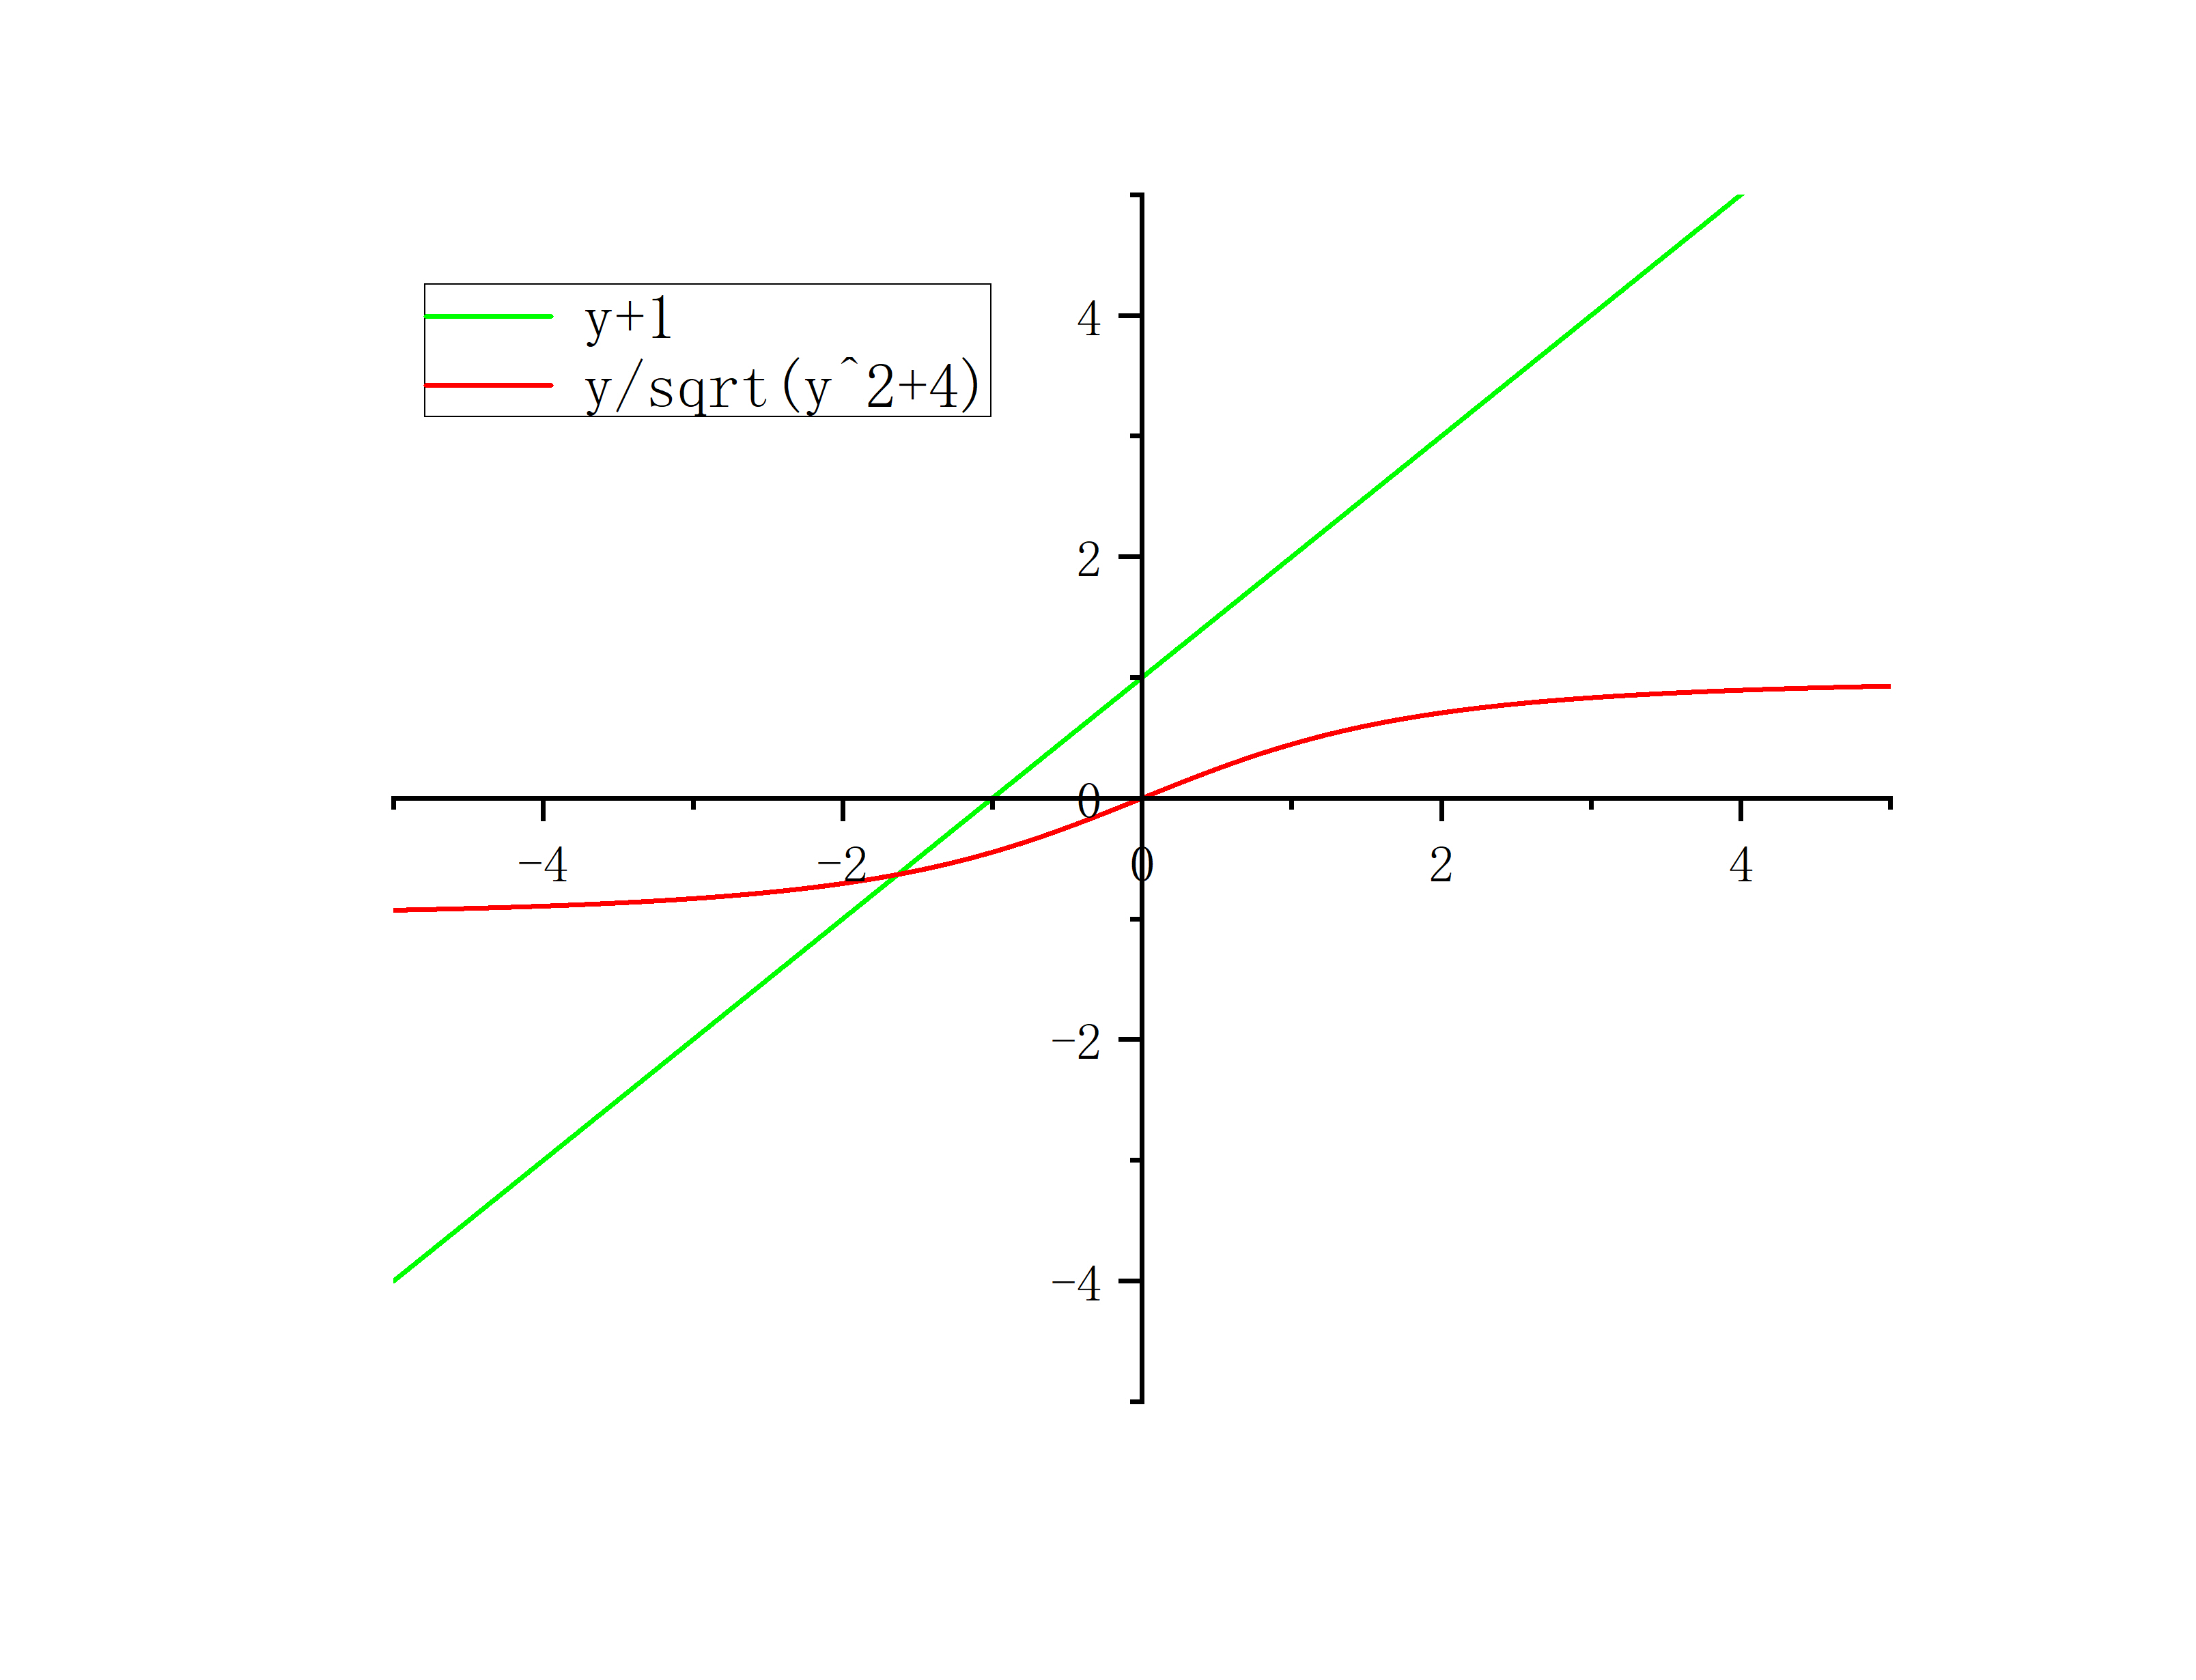
\includegraphics[width=0.6\textwidth]{极值点讨论示意图1.jpg}
        \caption{极值点讨论示意图1}\label{极值点讨论示意图1}
    \end{figure}

    当$\wx=0$时,可以根据物理图景知道,无论$\wg$如何取值,一定有两个极值点(考虑悬点固定并可额外施力的情况)。首先,y<0一定有一个平衡位置,
    此时对应弹簧自然下垂。当$y\ge0$时,对应弹簧撑起圆环,如果$\wg$不太大,弹簧可以撑起圆环,那么y>0有一个平衡位置;如果$\wg$过大
    以至于弹簧压缩到长度为0仍不够平衡重力,那么悬挂点一定会补偿一定的支持力,使得圆环静止在y=0处。

    当$0<\wx<1$时,如下图所示,f和h可能有1,2,3个交点。

    \begin{figure}[H]
        \centering
        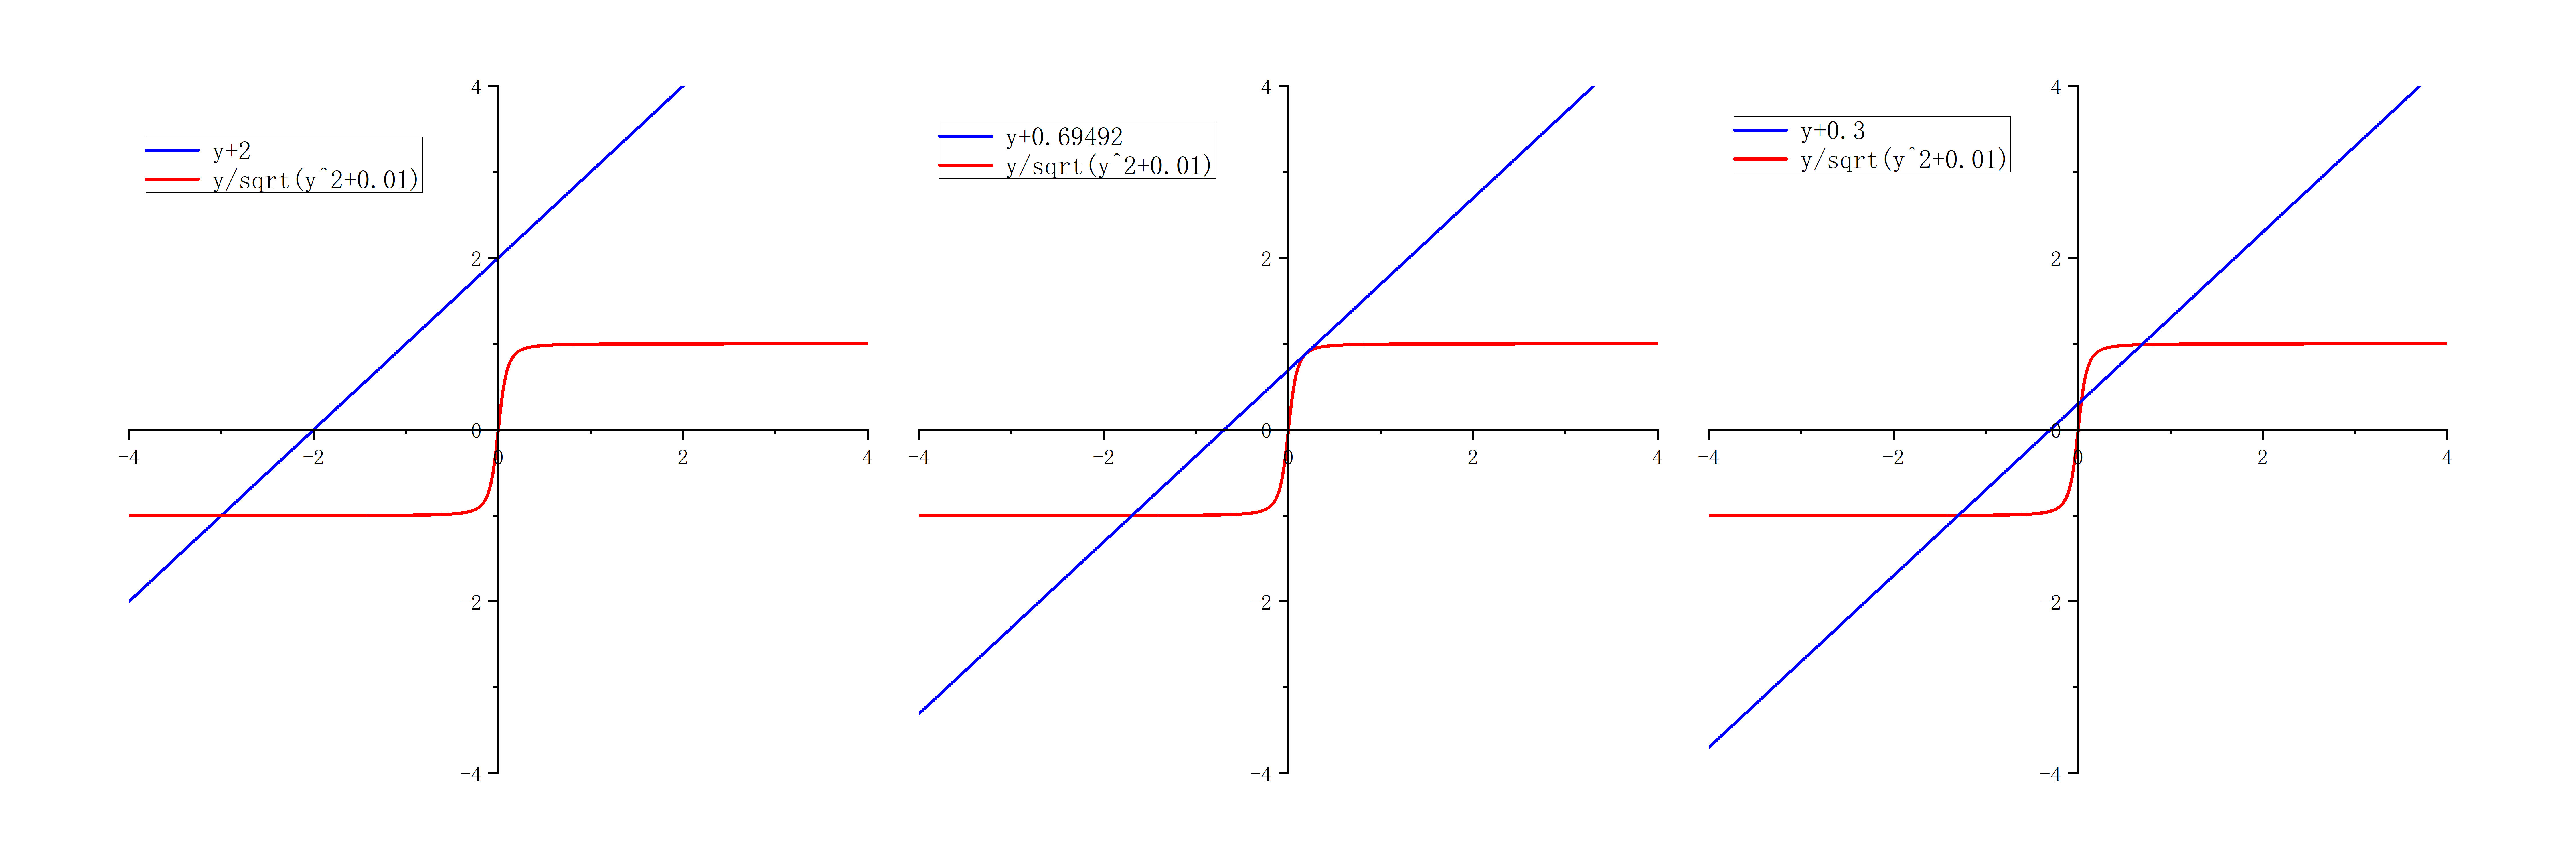
\includegraphics[width=0.9\textwidth]{极值点讨论示意图2.jpg}
        \caption{极值点讨论示意图2}\label{极值点讨论示意图2}
    \end{figure}

    当f,h有一个交点的时候,势函数有一个极值点,由势函数在正负无穷发散到无穷大,这个极值点一定是极小值点。

    当f,h有三个交点的时候,势函数有三个极值点,由势函数在正负无穷发散到无穷大,这三个极值点一定是有两个极小值点,一个极大值点。

    当f,h有两个交点时,在左侧交点左右,f和h交叉,势函数导数变号,是极值点;右侧交点是切点,交点左右势函数导数不变号,不是极值点。
    类似一个交点时的分析,这个极值点是极小值点。

    由上述分析可知,f和h有两个交点是一个极小值和两个极小值的分界点,设此时$\wg=\wg_0$,则

    \begin{align}
        \begin{cases}
            0\le\wg<\wg_0 & \text{f,h有三个交点,势函数有两个极小值点}\\
            \wg\ge\wg_0 & \text{f,h有一或两个交点,势函数有一个极小值点}\\
        \end{cases}
    \end{align}

    我们下面需要求出$\wg_0$同x的依赖关系。

    临界点f和h相切,切点满足$f'=h',f=h$,即
    
    \begin{align}
        \begin{cases}
            1=\frac{\wx^2}{(\wx^2+\wy^2)^\frac{3}{2}}\\
            \wy+\wg=\frac{\wy}{\sqrt{x^2+y^2}}
        \end{cases}
    \end{align}\label{第一问切点方程}
    
    于是对于任意x,在[0,1]中解出
    方程$(x^2+y^2)^3-x^4=0$的解y,再把x和y代入$\wg=\frac{\wy}{\sqrt{x^2+y^2}}-\wy$,即可得到给定x对应的g。

    在(0,1)每0.0001取一个点,输出对应的切点坐标y和临界g,具体代码实现见附件,运行代码,可以得到$"plot\_x-g\_data.txt"$中的数据。
    
    将x和g绘图得到下图。

    \begin{figure}[H]
        \centering
        \includegraphics[width=0.6\textwidth]{g-x图.jpg}
        \caption{g-x图}\label{g-x图}
    \end{figure}

    根据前面分析得到,第一象限内如图所示曲线以下的情况,系统有两个平衡位置;曲线以及以上的部分系统又一个平衡位置。

    由于体系水平和竖直方向的对称性,g-x图应当关于x轴和g轴轴对称,镜面对称延拓到全平面得到下图。

    \begin{figure}[H]
        \centering
        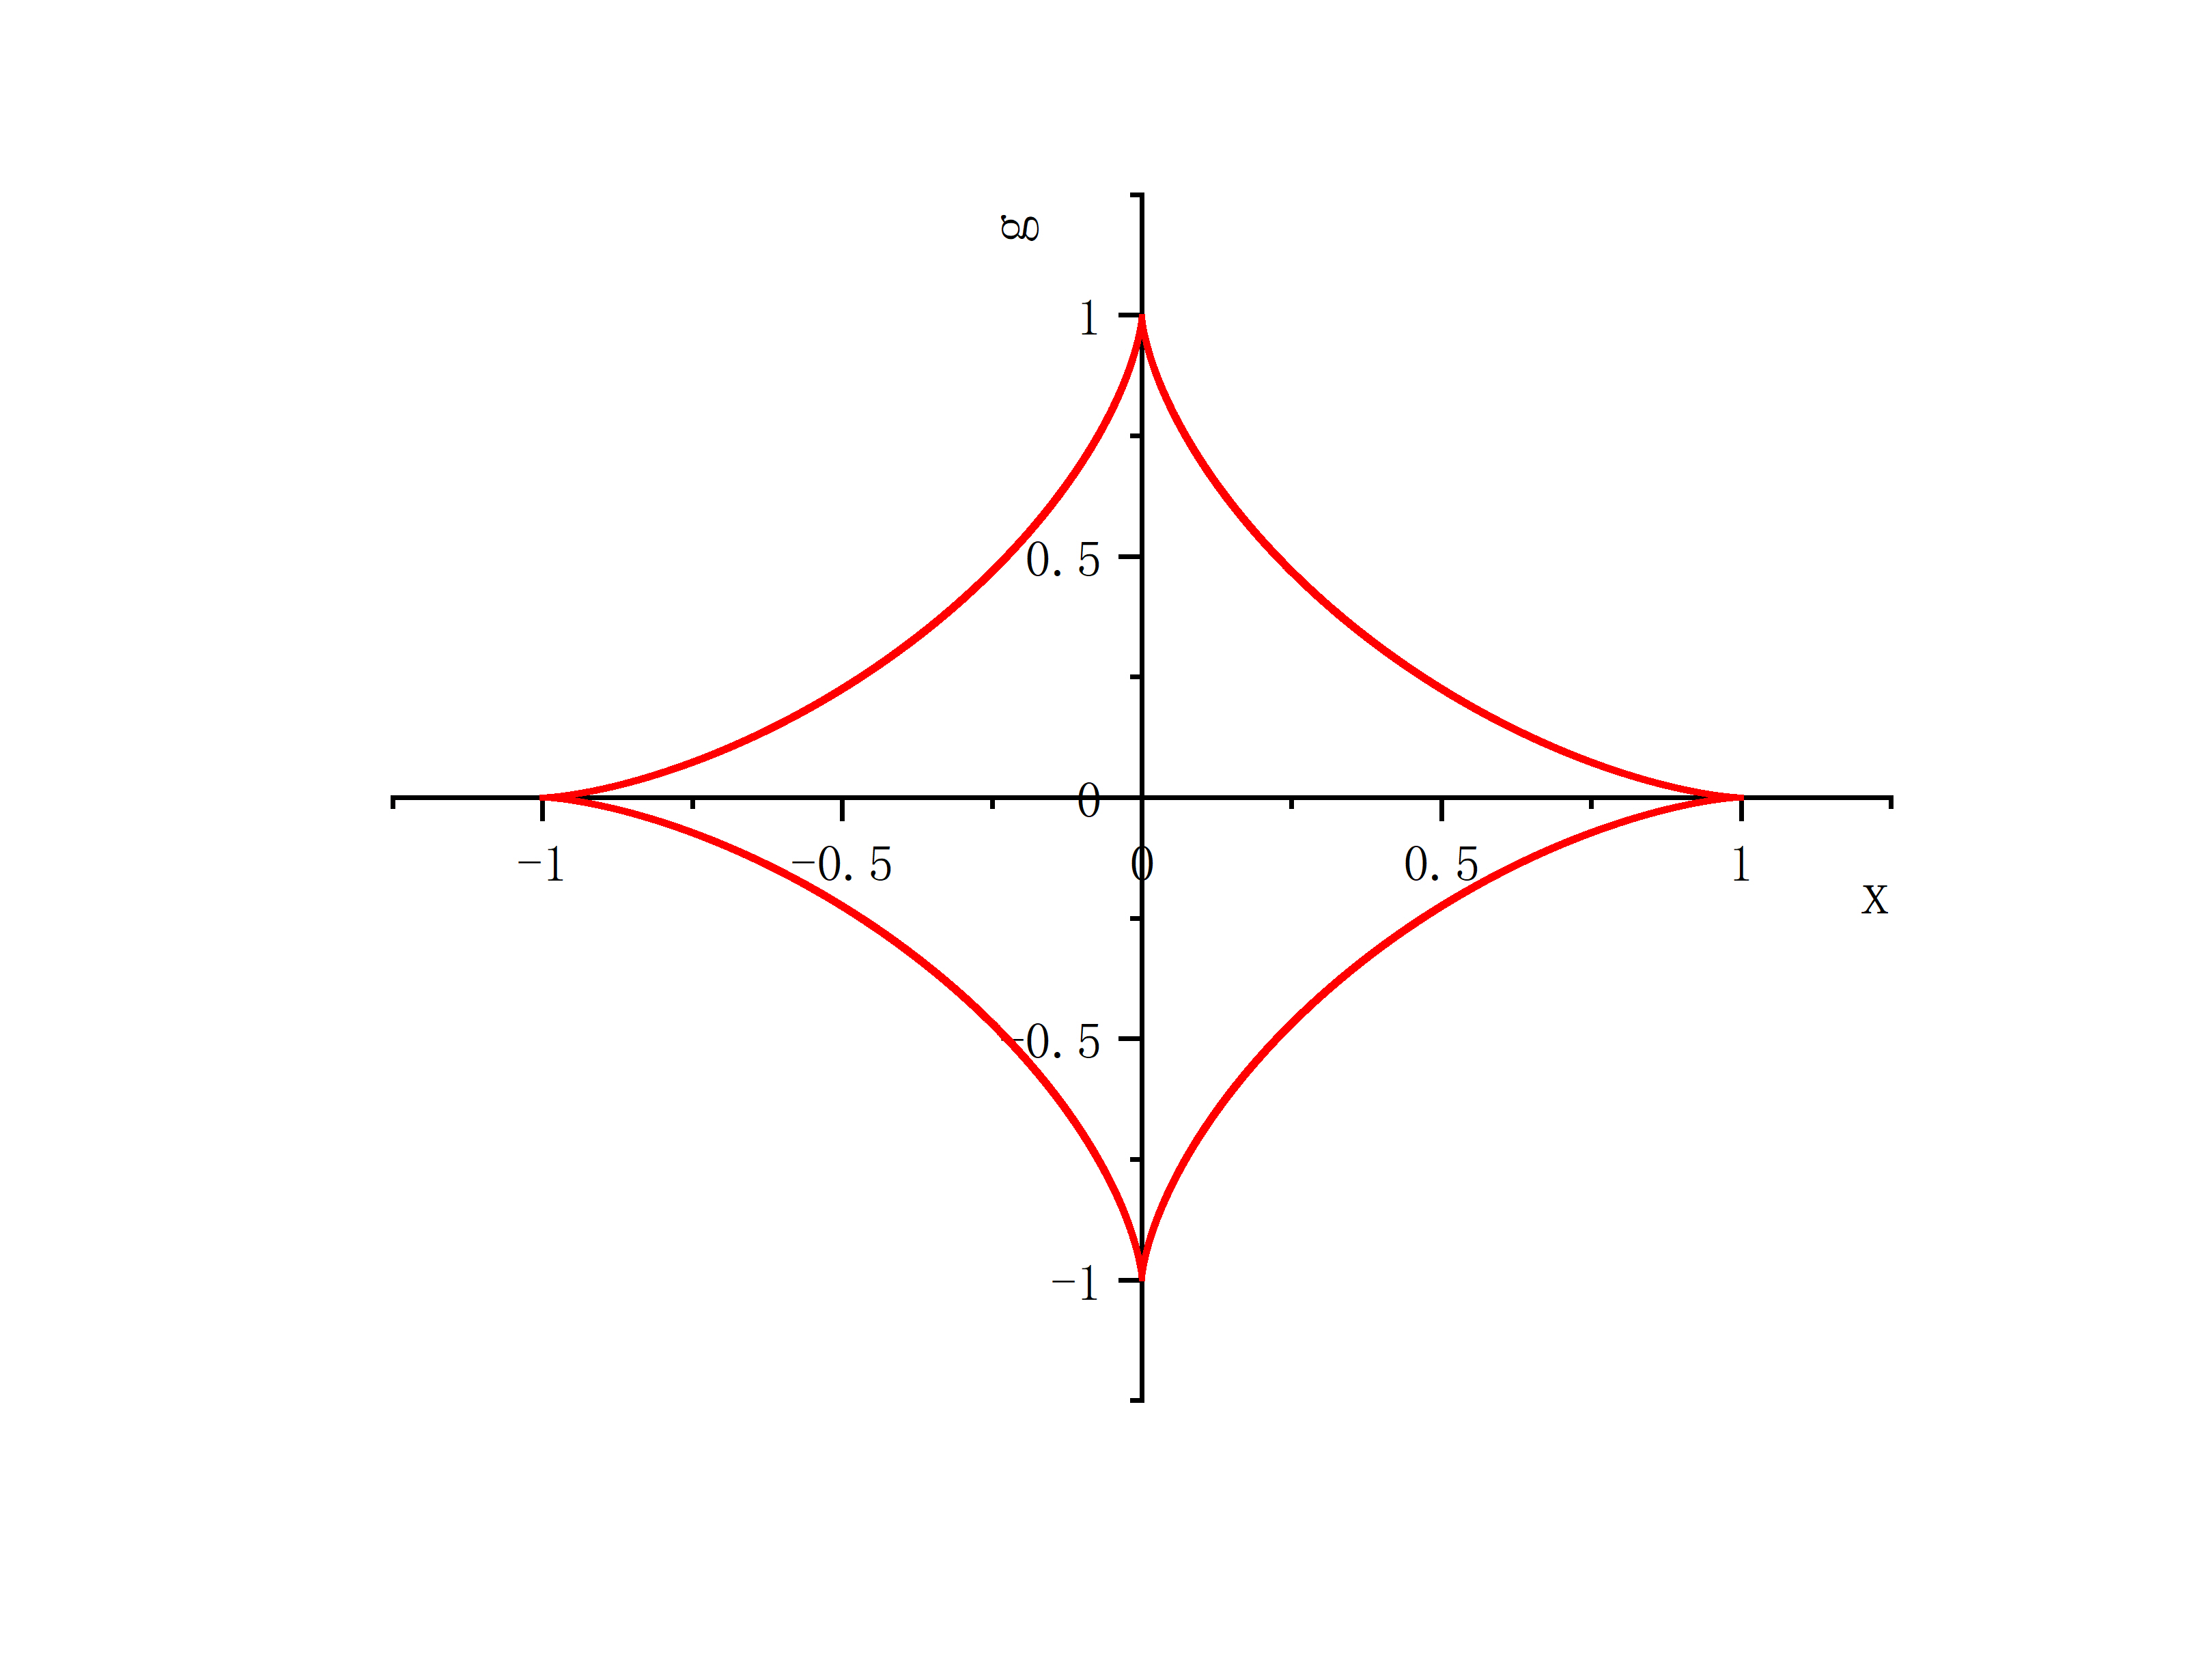
\includegraphics[width=0.6\textwidth]{g-x图-扩展.jpg}
        \caption{g-x图-扩展}\label{g-x图-扩展}
    \end{figure}

    曲线以内的点,系统有两个平衡位置,其他地方系统有一个平衡位置。

    \subsection{第2问}

    易知描述体系的哈密顿量和运动方程为

    \begin{align}
        H&=\frac{p_y^2}{2m}+\frac{1}{2}k(\sqrt{x^2+y^2}-l)^2+mgy\\
        \dot{p_y}&=-\frac{\partial H}{\partial y}=ky(\frac{l}{\sqrt{x^2+y^2}}-1)-mg\\
        \dot{y}&=\frac{\partial H}{\partial p_y}=\frac{p_y}{m}
    \end{align}

    我们首先需要对所有物理量进行无量纲化,规则如下:
    \begin{align}
        \wx=\frac{x}{l},\wy=\frac{y}{l},\wt=\sqrt{\frac{k}{m}}t,\wpy=p_y\frac{1}{ml}\sqrt{\frac{m}{k}},\wV=\frac{1}{l}\sqrt{\frac{m}{k}}v,\wV=\frac{V}{kl^2},\wH=\frac{H}{kl^2}
    \end{align}

    于是,体系的哈密顿量和运动方程化为

    \begin{align}
        \wH&=\frac{\wpy^2}{2}+\frac{1}{2}(\sqrt{\wx^2+\wy^2}-1)^2+\wg\wy\\
        \dot{\wpy}&=-\frac{\partial \wH}{\partial \wy}=\wy(\frac{1}{\sqrt{\wx^2+\wy^2}}-1)-\wg\\
        \dot{\wy}&=\frac{\partial \wH}{\partial \wpy}=\wpy
    \end{align}
    
    在本问中,有初始条件$\wpy=0,\wy=0.1$,参数演化形式为$\wg=0,\wx=2-\wv\wt$。

    题目要求对$\wv=1/4,1/16,1/64,1/256$
    分别讨论,下面笔者先给出计算方法,再给出不同$\wv$下的计算结果。\footnote{本报告中定义$N=\frac{1}{\wv}$,在源代码中会用到,特此说明。}

    \subsubsection{计算方法}
    \paragraph{相轨}

    解相轨需要求解一个如下的常微分方程组的初值问题

    \begin{align}
        \dot{\wpy}(\wx,\wy)&=\wy(\frac{1}{\sqrt{\wx^2+\wy^2}}-1) & \dot{\wy}(\wpy)&=\wpy\\
        \wpy_0&=0 & \wy_0&=0.1
    \end{align}

    这里采用蛙跳法求解。在确定迭代步长dt之后,用中点法计算出$\wt=0.5dt$之后的$\wpy_{\frac{1}{2}}$

    \begin{align}
        \wpy_{\frac{1}{2}}=\wpy_0+\frac{1}{2}dt\cdot\dot{\wpy}(\wx(\frac{1}4{dt}),\wy_0+\dot{\wy}(0)\cdot\frac{1}{4}dt)
    \end{align}

    于是可以实现蛙跳,得到$\wy_0,\wy_1,\wy_2...\wpy_\frac{1}{2},\wpy_\frac{3}{2},\wpy_\frac{5}{2}...$,迭代公式如下

    \begin{align}
        \wy_{n+1}&=\wy_n+dt\cdot\wpy_{n+\frac{1}{2}}\\
        \wpy_{n+\frac{3}{2}}&=\wpy_{n+\frac{1}{2}}+dt\cdot \wy_n(\frac{1}{\sqrt{\wx^2(\wt)+\wy_n^2}}-1)
    \end{align}

    由于绘制相图需要对应的$\wy$和$\wpy$,我们可以在每次迭代中线性近似,取$\wpy_{n+1}=(\wpy_{n+\frac{1}{2}}+ \wpy_{n+\frac{3}{2}})/2$得到。

    \paragraph{J-x关系图}

    根据绝热不变量的定义,计算时需要将缓变参数固定。也就是说,这里任取一个时刻$\wt$,我们已经算过这个时刻的$\wy,\wpy$,这个时候需要锁定x,并且以这个时刻的位置和动量为初始条件,
    让系统作周期性震荡,进而在它的相空间中计算绝热不变量。

    进而,问题简化为:给定x,给定初值条件$\wy_0,\wpy_0$,计算$\frac{1}{2\pi}\oint \wpy d\wy$。

    我们可以根据g=0的条件对积分进行简化。

    \begin{figure}[H]
        \centering
        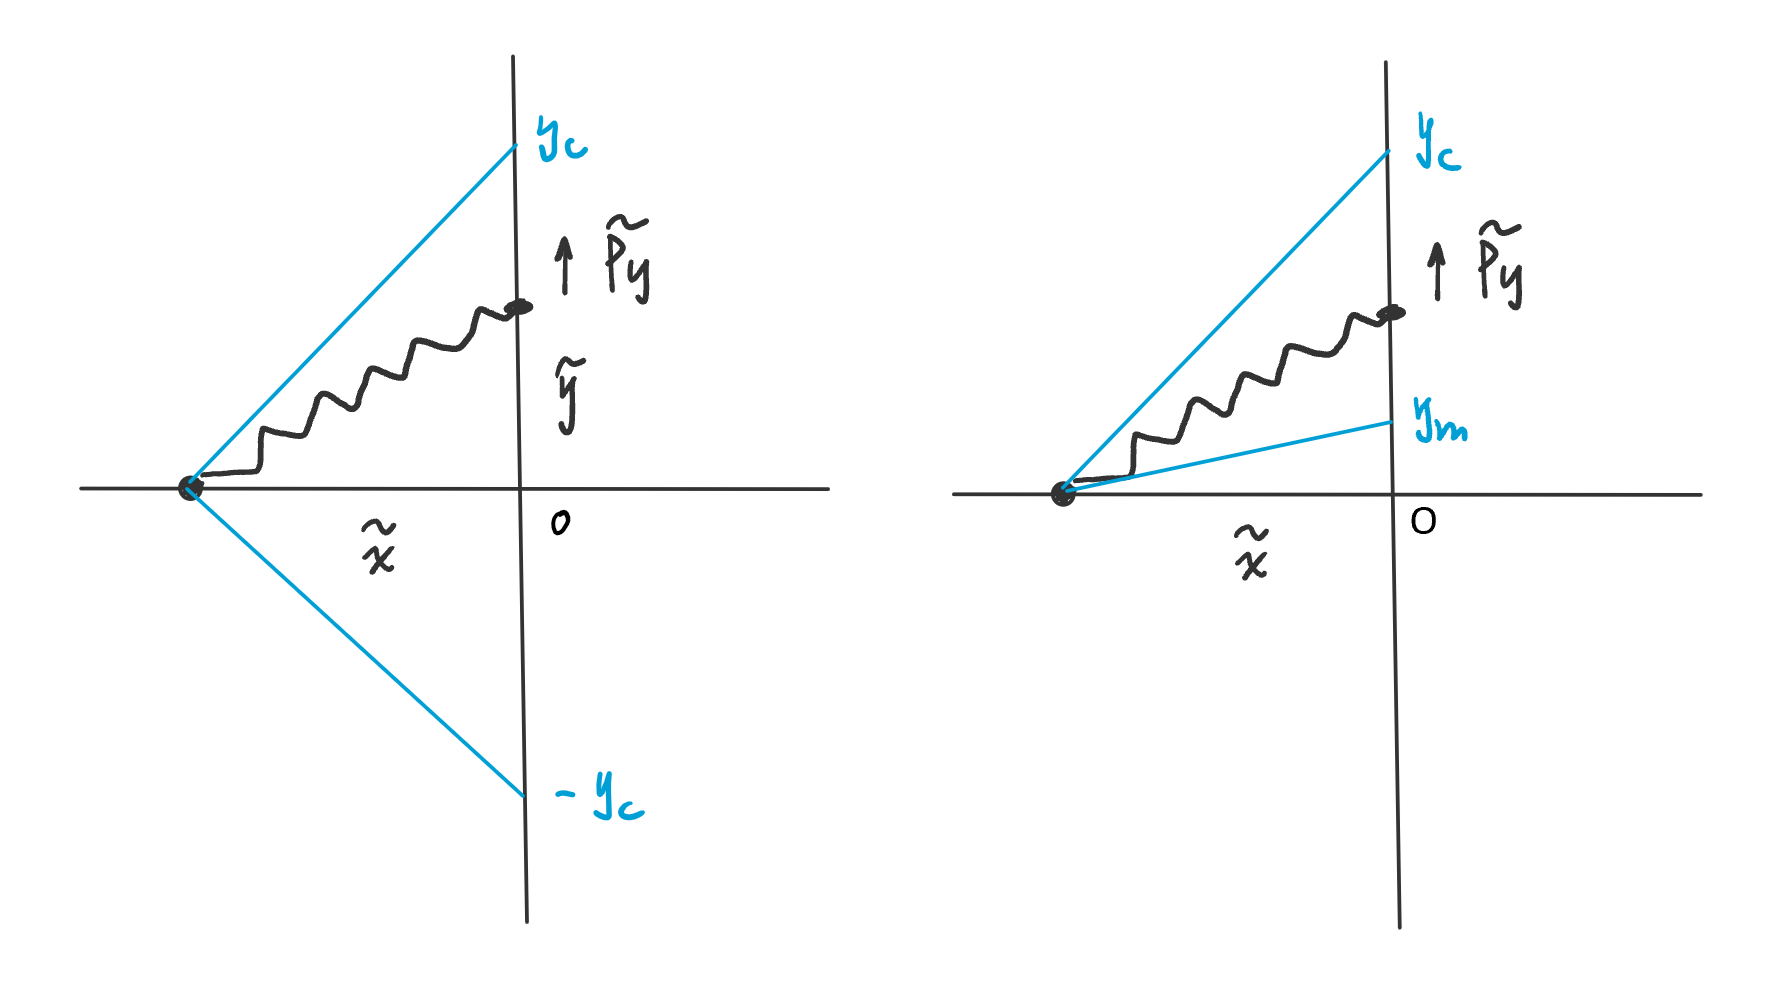
\includegraphics[width=0.6\textwidth]{J-x计算方法示意图.png}
        \caption{J-x计算方法示意图}\label{J-x计算方法示意图}
    \end{figure}

    如图所示,g=0时只可能有这两种运动模式。当振子能量较大的时候,可以越过中点O,那么震荡是左图形式;否则,振子不能越过中点O,震荡是右图形式。而且,在右图这种情况中,
    振子被限制在上半空间和下半空间是完全对称的,不妨都转化为在上半空间进行计算;而在左图情况中,相图一定关于原点中心对称。于是,我们不妨把初值条件都取绝对值。
    即$\wy_0\ge0,\wpy_0\ge 0$

    如何判断能否越过中点O呢?我们通过初值条件算出体系能量H,这个能量守恒。如果H大于y=0时的势能,那么振子越过中点;否则,振子不越过中点。

    我们还需要得到动量为0的点作为积分上下限。上限$\wy_c$两种情况是一致的,都是求解$\wH-\wV(\wy)=0$在$[\wy_0,+\infty]$中的根(一般正无穷会取预估的上界)。
    而右图情况还需要求解$\wy_m$,只需要求解$\wH-\wV(\wy)=0$在$[0,\wy_0]$中的根即可。

    进而,可以用下式积分得到J

    \begin{align}
        \begin{cases}
            \text{左图}& J=\frac{2}{\pi}\int_0^{y_c}p_ydy\\
            \text{右图}& J=\frac{1}{\pi}\int_{y_m}^{y_c}p_ydy
        \end{cases}
    \end{align}

    \subsection{图像展示}
    \textbf{两部分代码可以组合,具体见附录,运行结果见“q2-1.txt”,“q2-2.txt”,“q2-3.txt”,“q2-4.txt”}
    \footnote{编号为1,2,3,4分别对应$\wV=1/4,1/16,1/64,1/256$时输出文件,本报告中txt文件无特别说明,均表示这个含义。}

    下面左图是相轨,右图是J-x图。

    \begin{figure}[H]
        \centering
        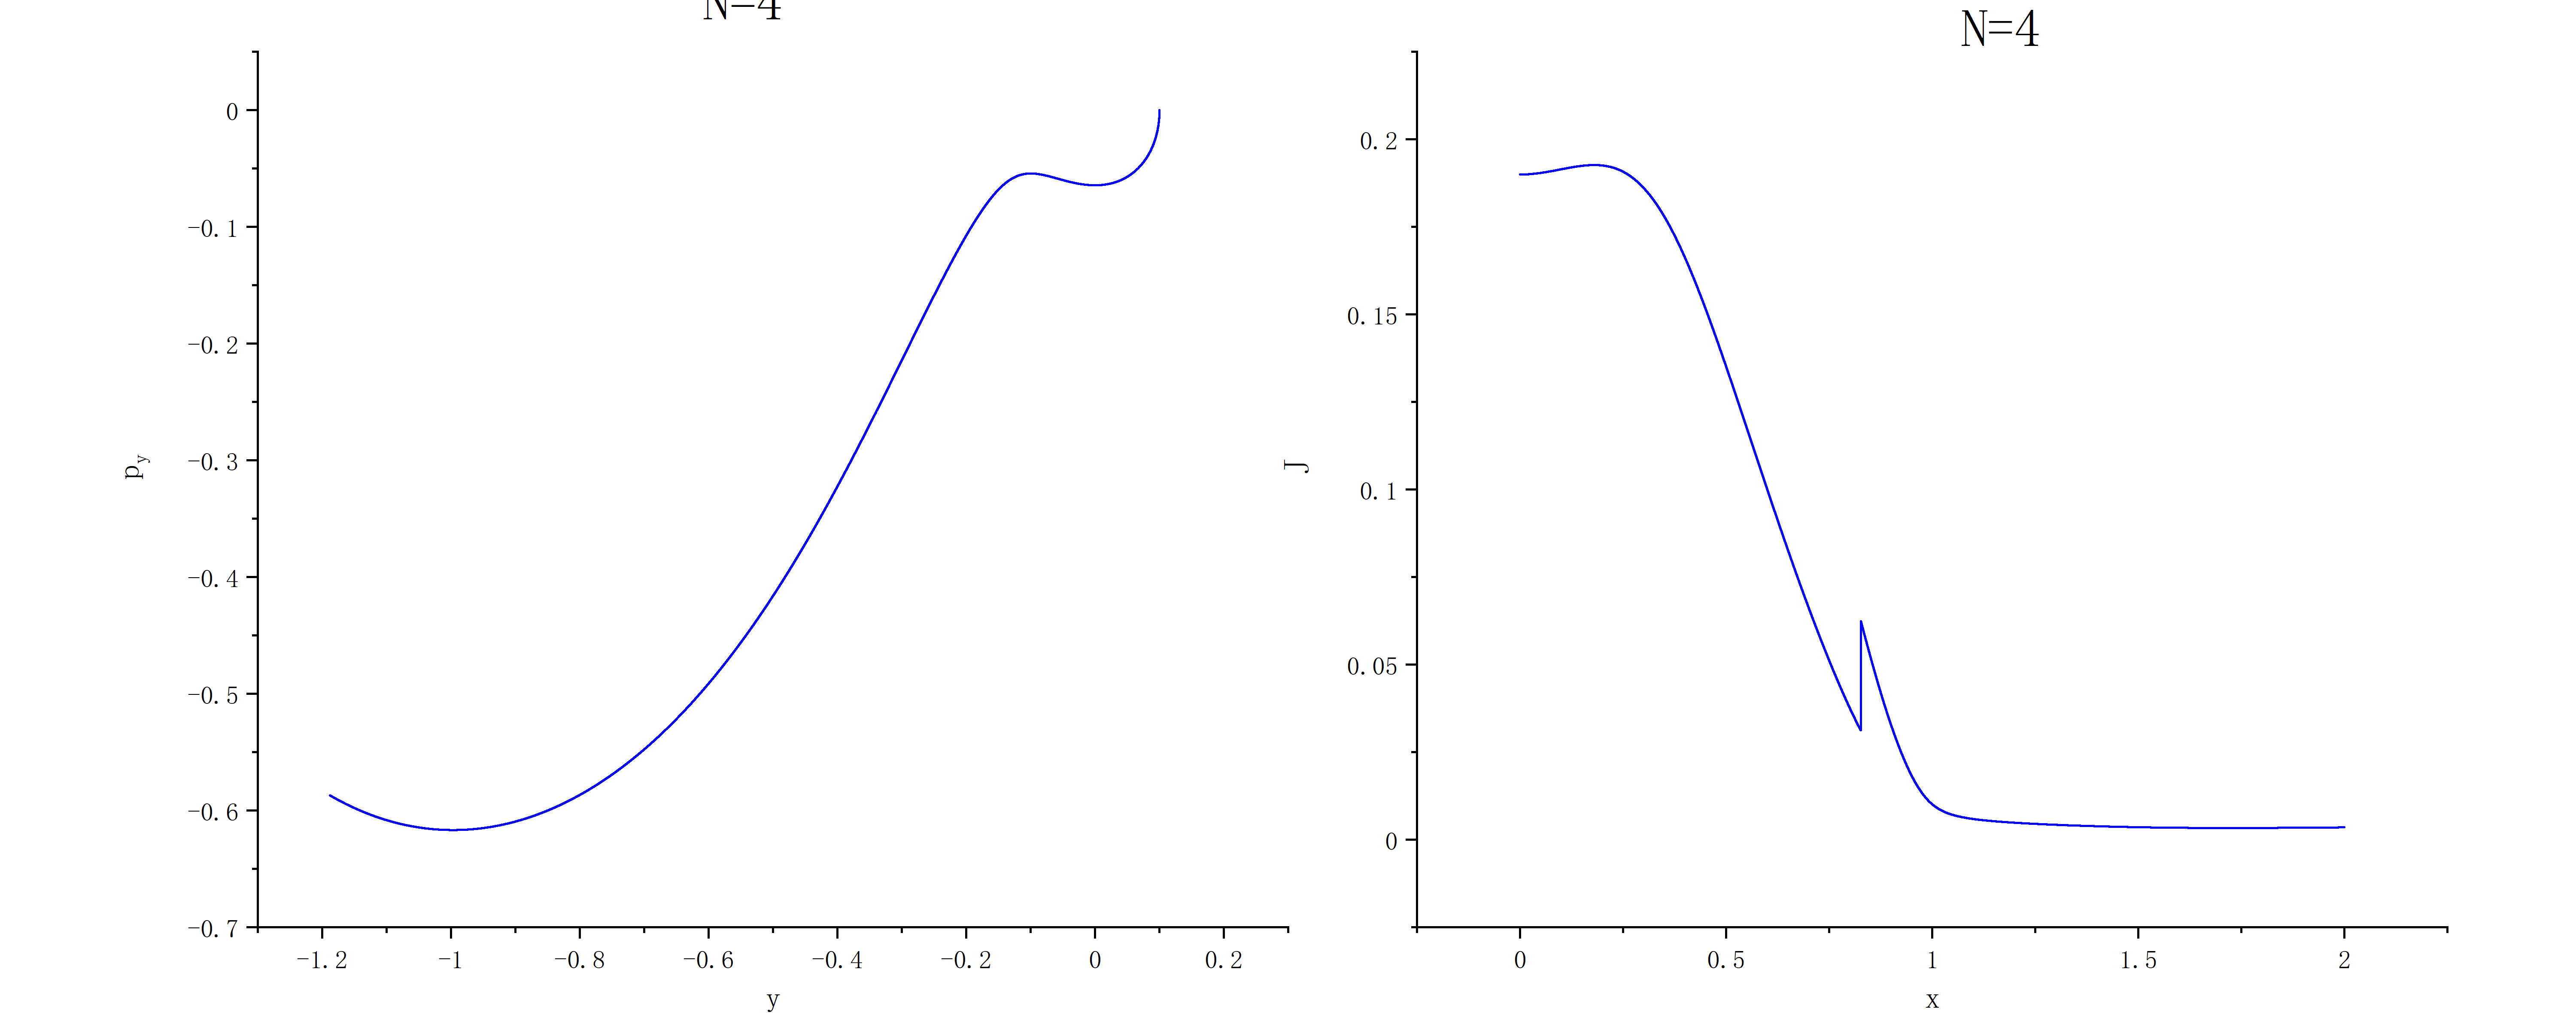
\includegraphics[width=0.9\textwidth]{q2-N=4.jpg}
        \caption{q2-N=4}\label{q2-N=4}
    \end{figure}

    \begin{figure}[H]
        \centering
        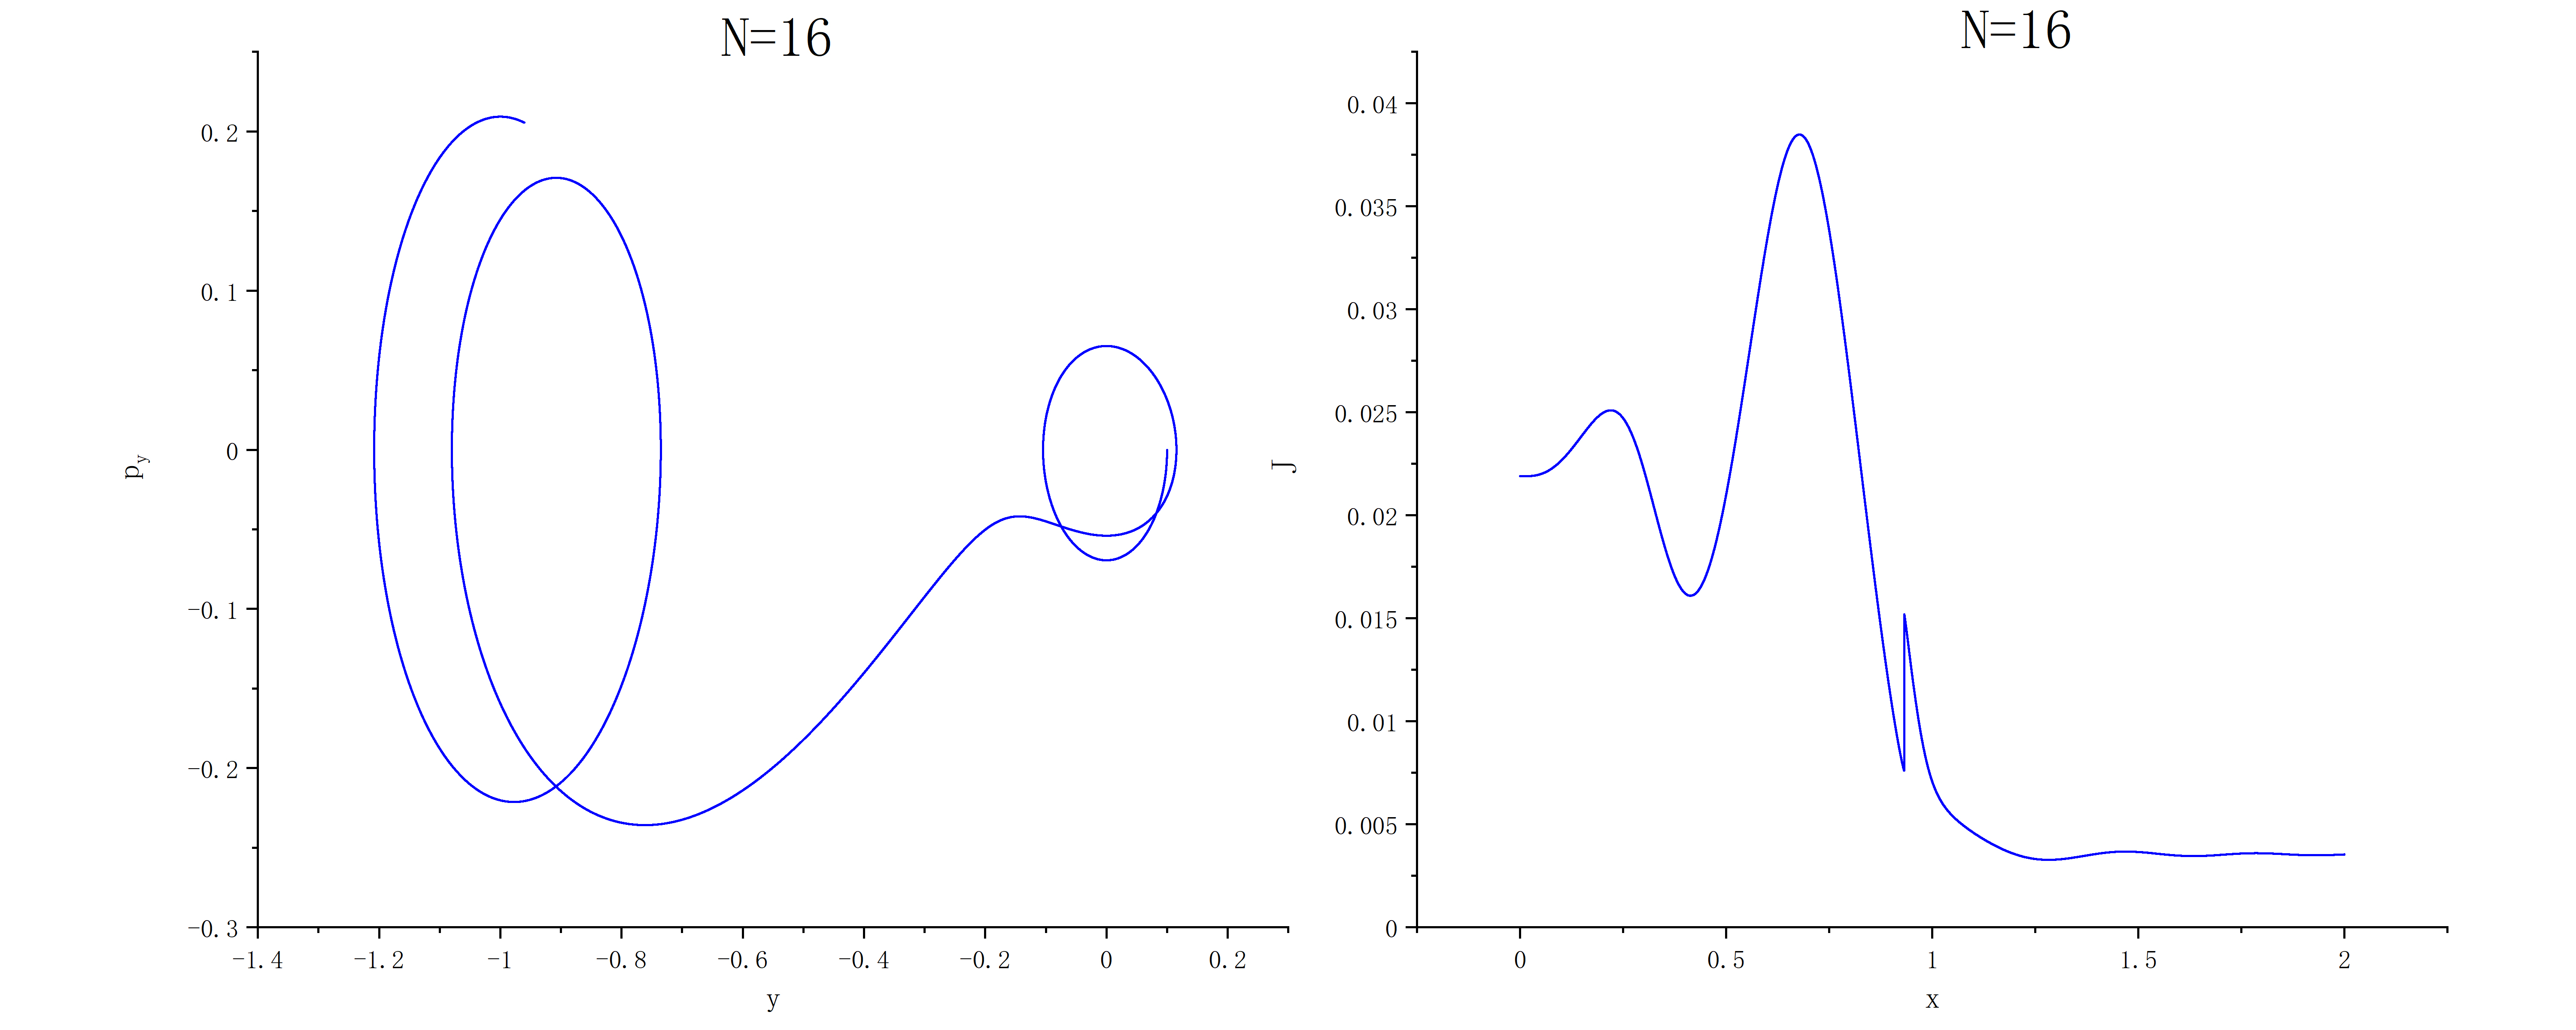
\includegraphics[width=0.9\textwidth]{q2-N=16.jpg}
        \caption{q2-N=16}\label{q2-N=16}
    \end{figure}

    \begin{figure}[H]
        \centering
        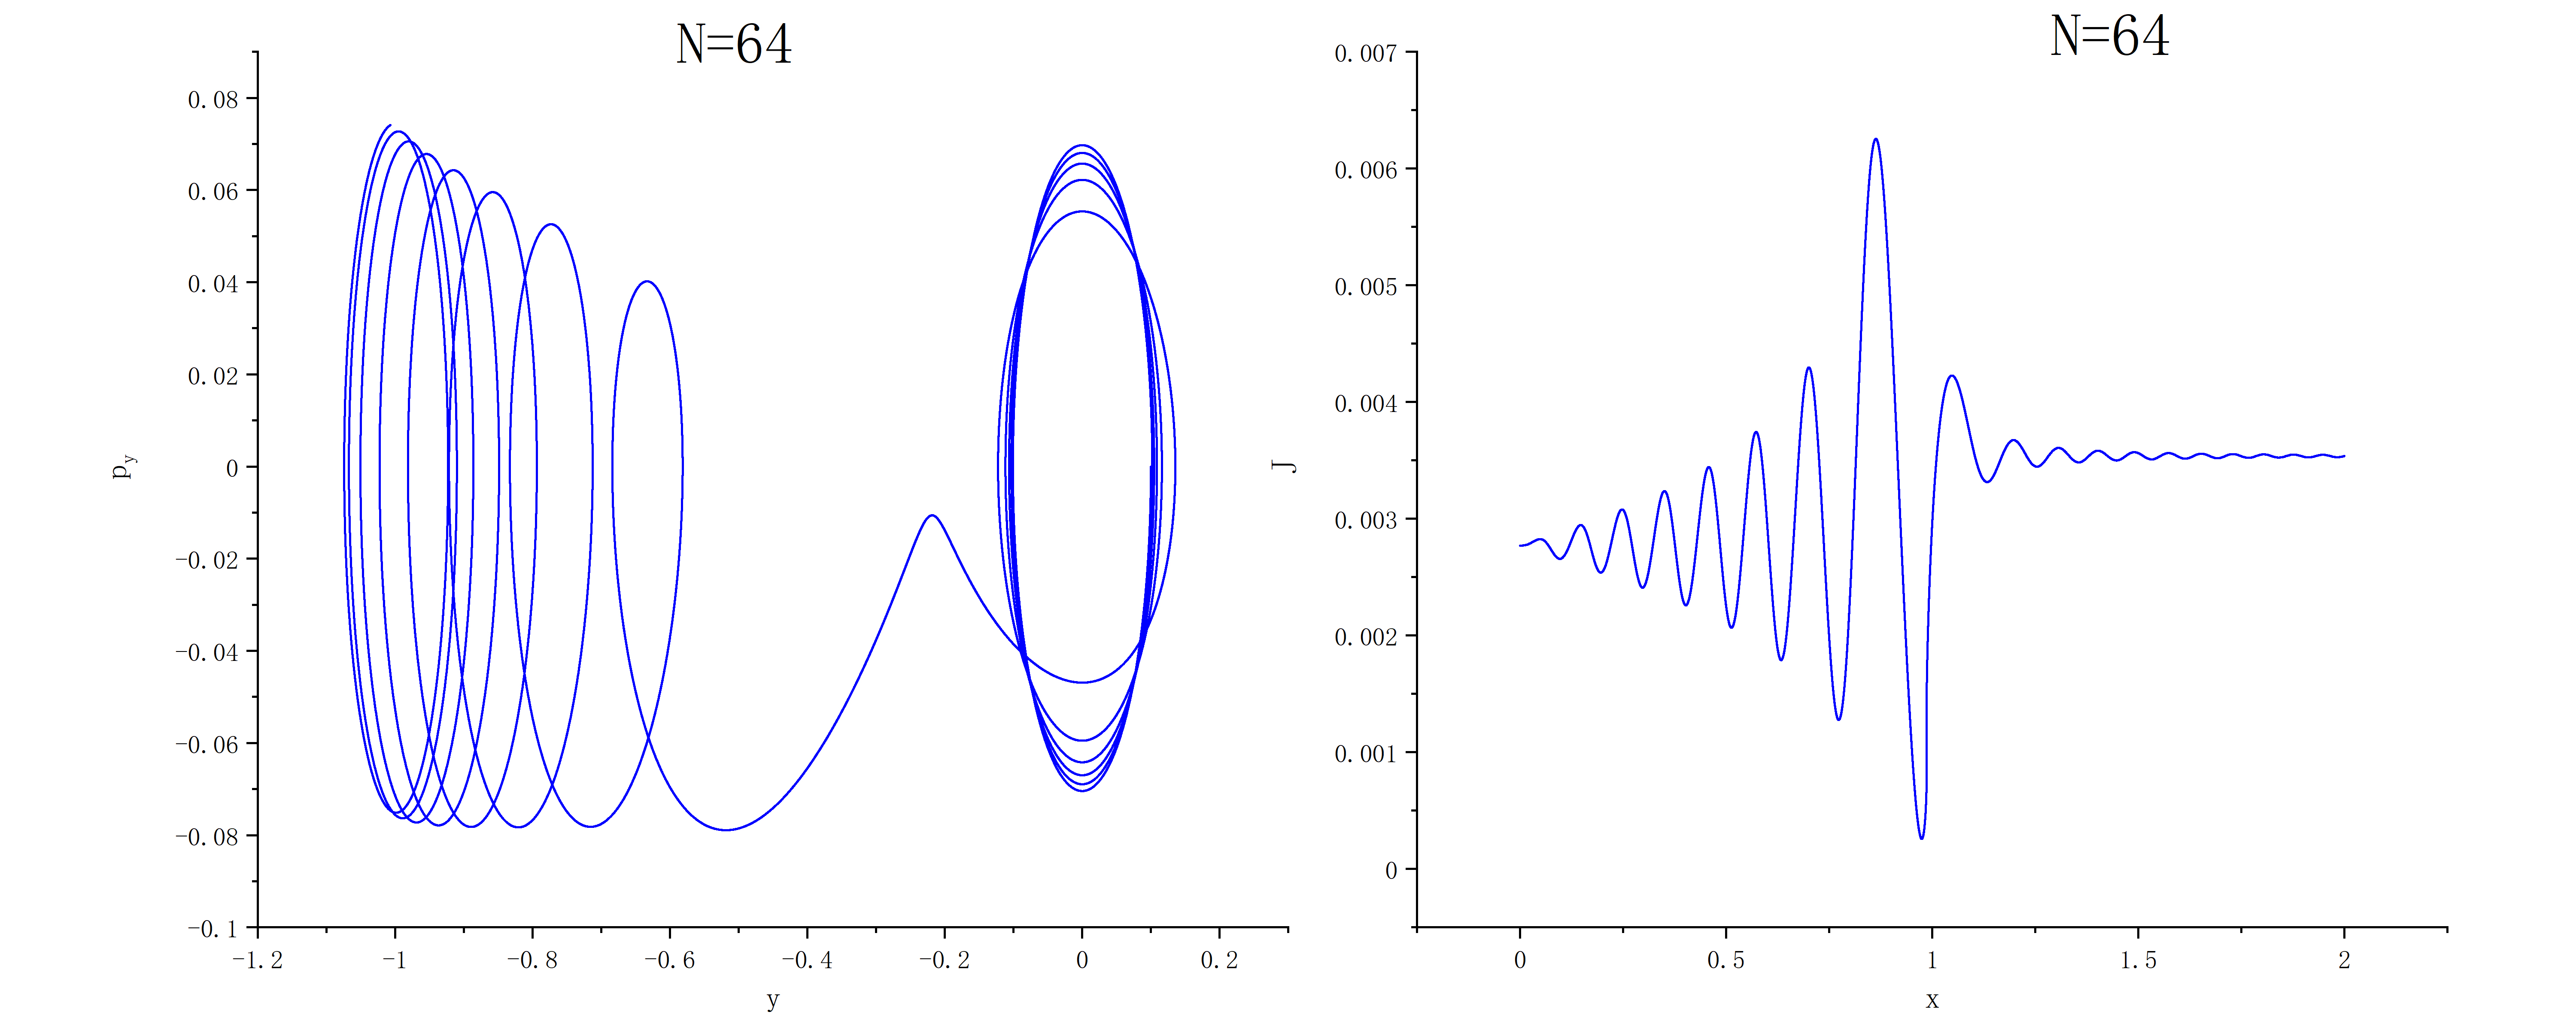
\includegraphics[width=0.9\textwidth]{q2-N=64.jpg}
        \caption{q2-N=64}\label{q2-N=64}
    \end{figure}

    \begin{figure}[H]
        \centering
        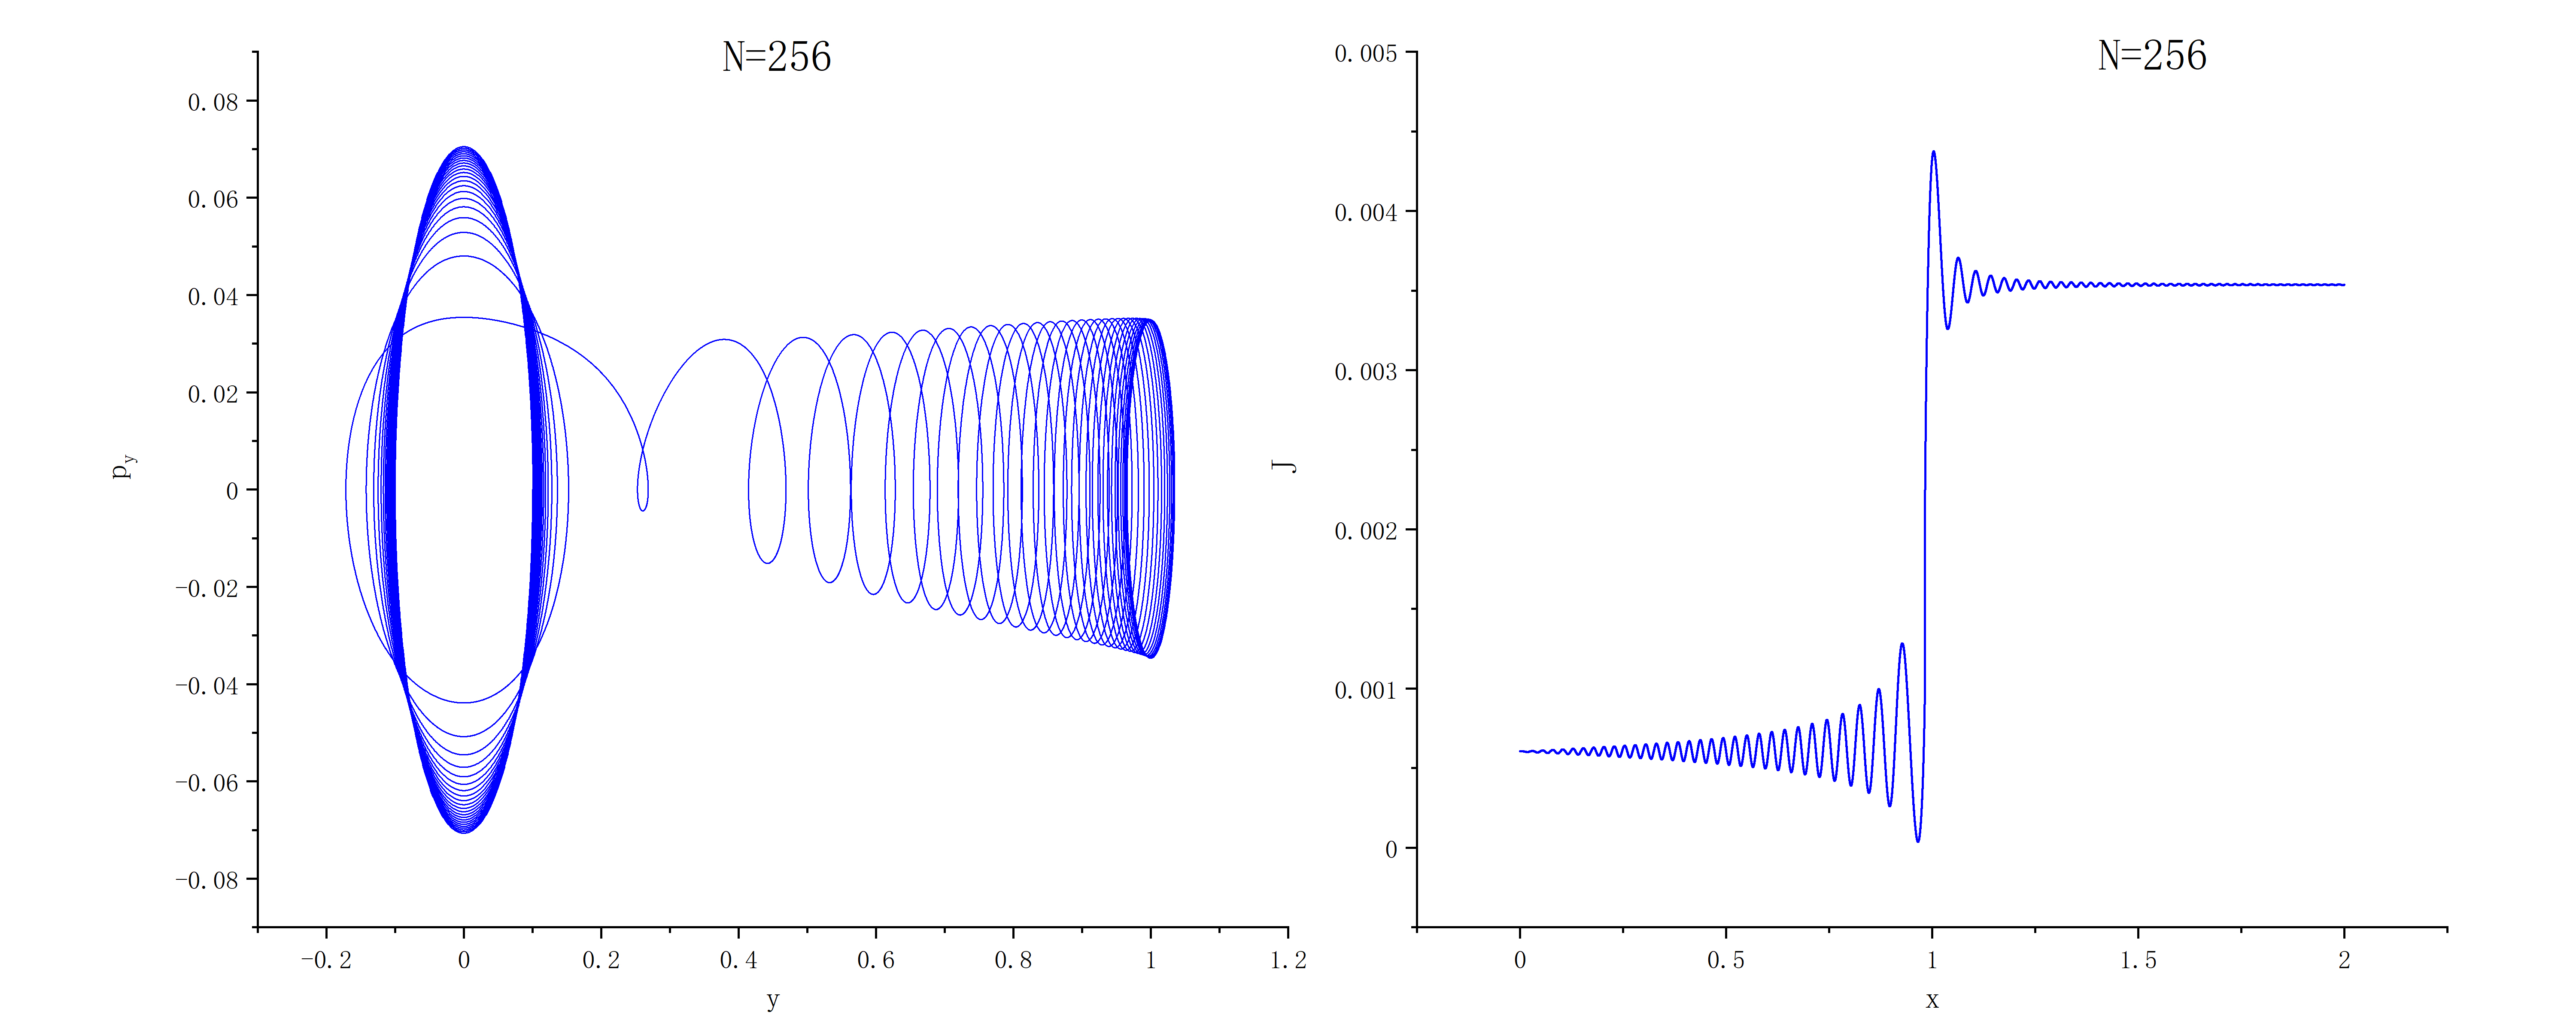
\includegraphics[width=0.9\textwidth]{q2-N=256.jpg}
        \caption{q2-N=256}\label{q2-N=256}
    \end{figure}

    可以看出,当N逐渐变大时(x变化越缓慢),J越趋向于一个不随x变化的常数(可能有阶跃,如图\ref{q2-N=256})。

    
    \subsection{第3问}

    本问初值条件变为$\wpy_0=0,\wy_0=-2$,缓变参数为$\wx=0.2,\wg=2\cos{(2\pi\wt/N)}$,要求讨论N=4,16,64,256时的相轨和J-g图象。

    \subsubsection{计算方法}

    \paragraph{相轨}

    相轨计算与第二问完全相同。

    \paragraph{J-g图}

    由于g非零,上下空间的对称性破缺,进而不再能用第二问的方法计算J值。需要将第二问的方法一般化,即求总能量H和势函数的两交点坐标$y_1,y_2$,
    再由积分$\frac{1}{\pi}\int_{y_1}^{y_2}\wpy d\wy$求出J。

    总能量可以由初值条件轻松算出,但是,交点的求解遇到了势函数多极值点的问题。根据第一问的结论(图\ref{g-x图}),x=0.2
    、g在[-2,2]中,存在一个$g_0\approx0.53375$使得$|g|<g_0$时势函数有两个极小值,此外有一个极小值。

    当势函数有一个极小值时,求解是容易的。这时需要先求出势函数极小值点,然后在极小值两侧分别找到交点,亦即,积分上下限$y_1,y_2$。

    当势函数有两个极小值时,就存在如下图所示的三种情况。

    \begin{figure}[H]
        \centering
        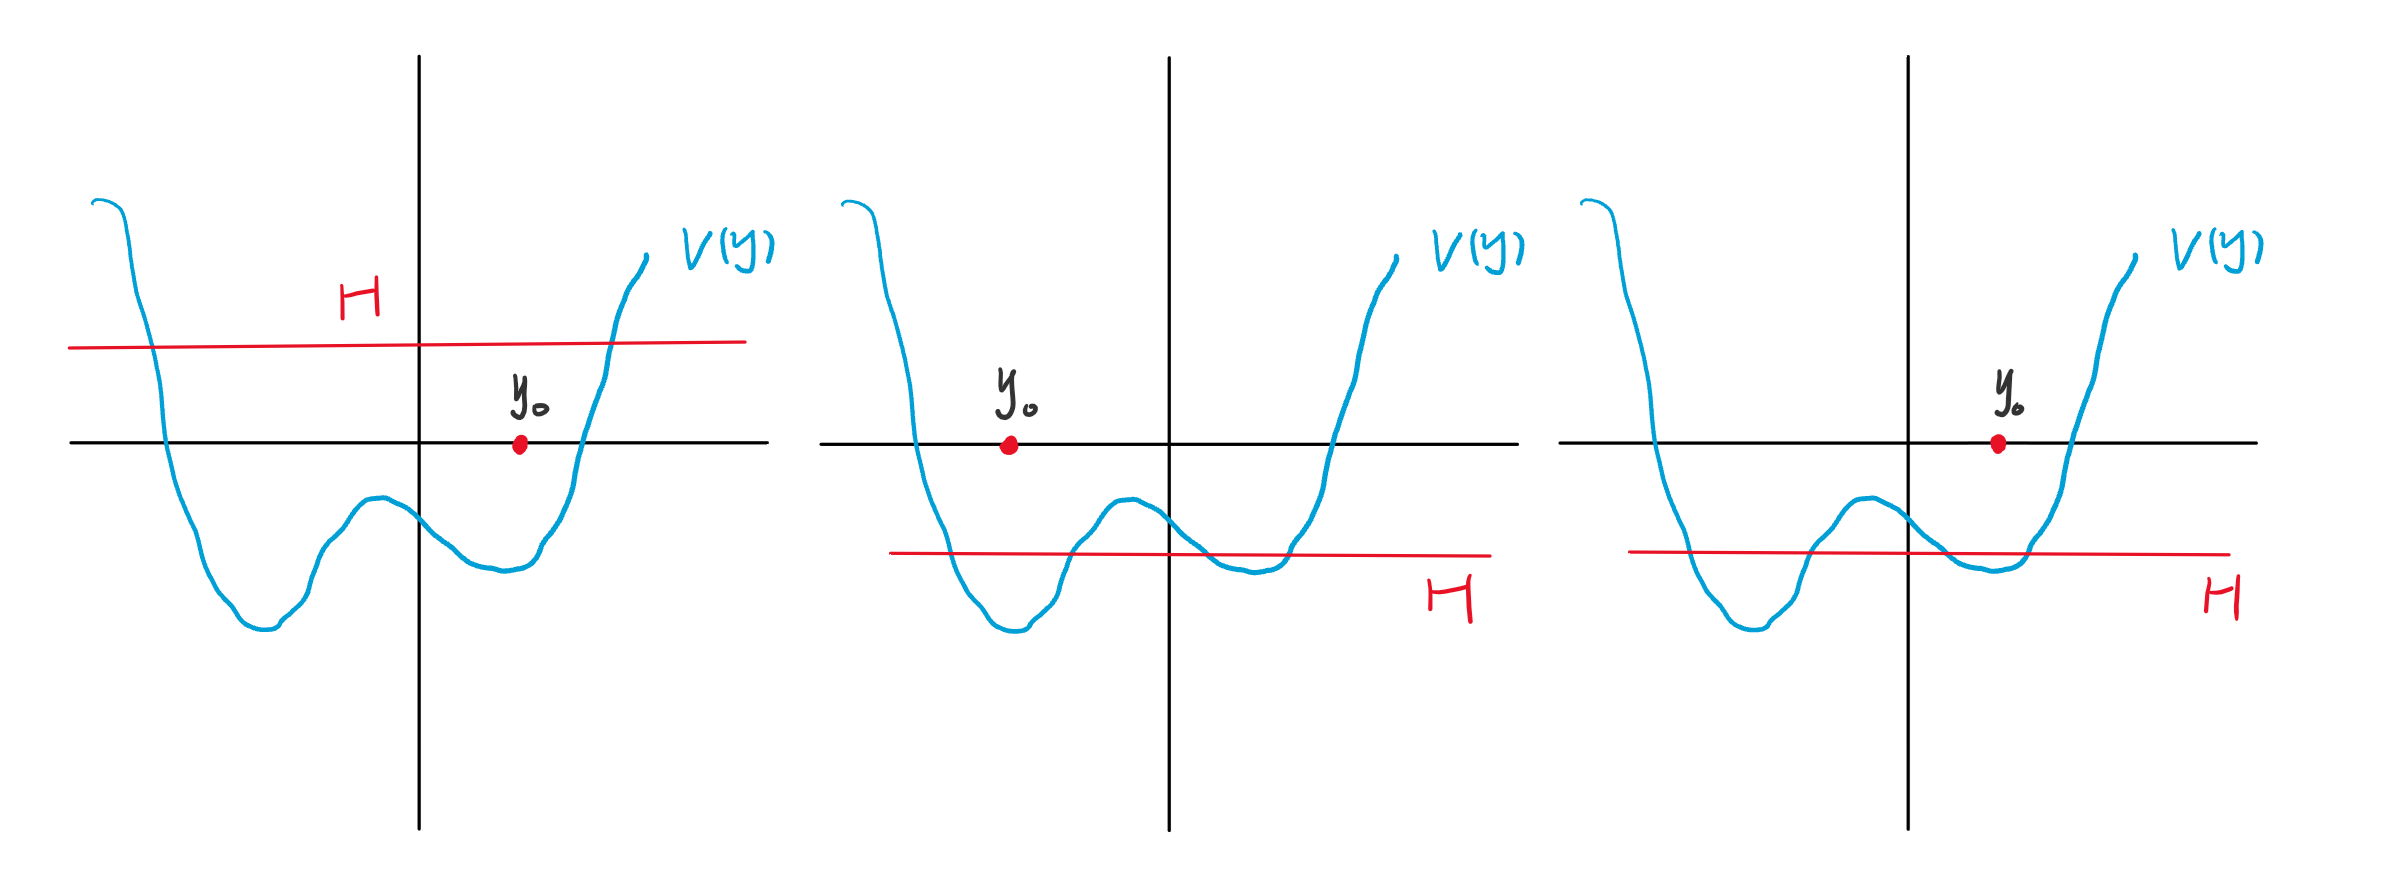
\includegraphics[width=0.9\textwidth]{J-g计算方法示意图.png}
        \caption{J-g计算方法示意图}\label{J-g计算方法示意图}
    \end{figure}

    如果能量比较高,如左图情形,球根方法将类似一个极值点情形。如果能量较低,势函数就和总能量有4个交点!这会在求根过程中给求根算法带来困惑,我们需要摒弃粗犷的
    求根区间,找到更加精确的求根区间。而且这个时候振子在哪个“谷”中振荡完全取决于初值条件,如中、右图所示。初值在哪个谷中,振子就在哪个谷中振荡,$y_1,y_2$
    就取哪个谷里的交点。

    种种麻烦表明,我们需要对势函数的变化趋势有更加细致的掌握。如果能够知道势函数两个极小值点和极大值点的坐标,问题就会方便很多。试看,如何区别左图和中、右图呢?我们
    比较总能量和极大值点处势函数取值,若大于,则是左图情形;否则,中右图情形。如何区别中和右图呢?我们比较初值$\wy_0$和极大值点,如果初值y在极大值点左侧,就是中图情形;
    否则,右图情形。

    求出两个极小值点和极大值点更有利于我们求根。
    
    如果我们从左到右依次叫三个极值点“Ymin2”“Ymax”“Ymin1”,那么左图情形我们可以分别在区间$[-\infty,Ymin2]$和
    $[Ymin1,\infty]$中求解。中图情形我们可以在区间$[-\infty,Ymin2]$和$[Ymin2,Ymax]$中求解。右图情形我们可以在区间$[Ymax,Ymin1]$和$[Ymin1,\infty]$中求解。
    容易证明,本题势函数在以上各区间单调,根据求根算法的性质,极大的增强了程序健壮性。(一般$\infty$取经验上的一个上界)

    那么,任给x和g如何求势函数两个极小值点和一个极大值点呢?这需要用到第一问中的方法,将极值点的求解转化为两个函数图像的交点问题。

    \begin{figure}[H]
        \centering
        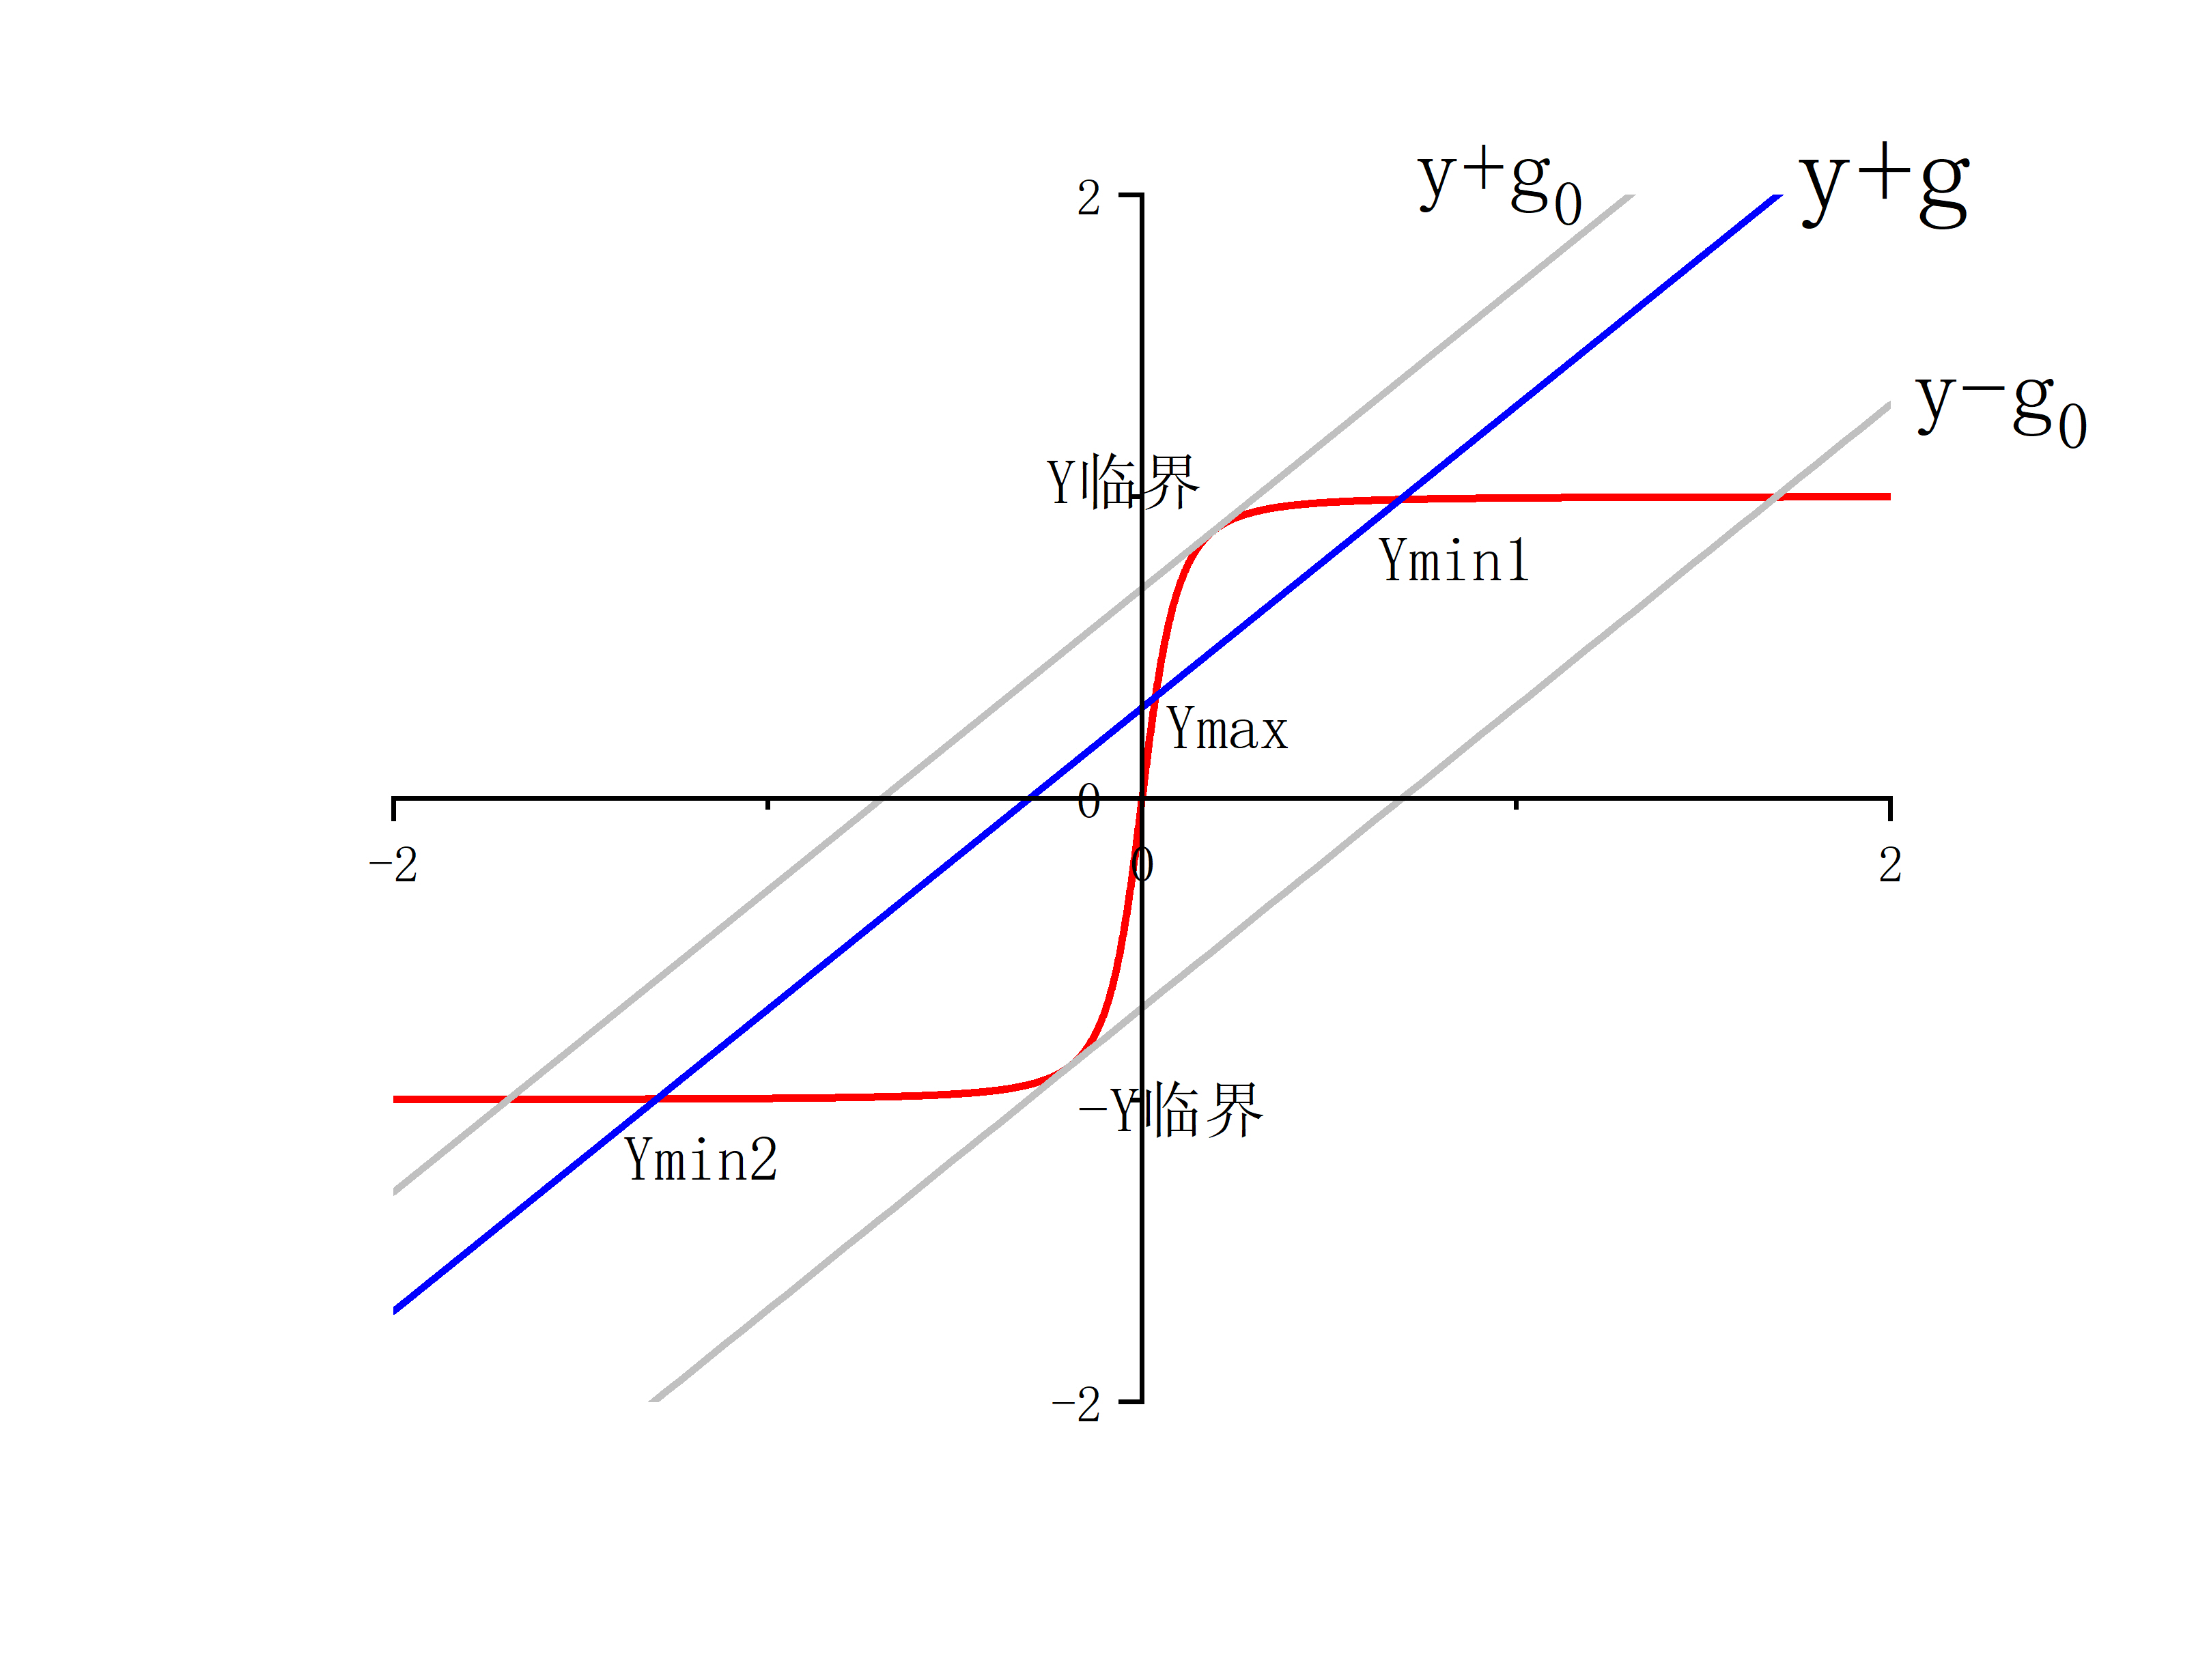
\includegraphics[width=0.6\textwidth]{q3极值点求法示意图.jpg}
        \caption{q3极值点求法示意图}\label{q3极值点求法示意图}
    \end{figure}

    
    如上图所示,本问中固定了x,于是
    红色的曲线就固定了,变化g的时候,三交点(对应三极值)情形对应蓝线,此时蓝线一定在两条灰线中间,而灰线是直线与红线的切线。第一问中已经得到,蓝线与红线的三个交点,两侧的
    是极小值点,中间的是极大值点。很直观地可以看出,如果记灰线和红线地切点为$\pm$Y临界,那么极大值点一定在两个临界点中间,极小值点分别在正负临界点之外。而第一问已经算过,
    x=0.2时,Y临界=0.277417932961286,因此分别在三个区间$[-\infty,-Y\text{临界}][-Y\text{临界},Y\text{临界}][Y\text{临界},\infty]$上利用求根算法,
    就可以求出Ymin2,Ymax和Ymin1。

    
    问题就此解决。总结一下计算方法:拿到一个x,g和一组初值条件$\wy_0,\wpy_0$;想要求振子相空间上下限$y_1,y_2$

    1、先用初值条件算总能量H

    2、判断:如果$|g|>g_0$,算势函数极小值点,在极小值点两侧求解H和势函数在极小值点两侧的交点即为$y_1,y_2$

    3、$|g|<g_0$,算势函数两个极小值点和一个极大值点。

    (1)如果H大于极大值点处势能,求解H和势函数在两个极小值两侧的交点即为$y_1,y_2$

    (2)否则:如果$\wy_0<$极大值点,在左边的谷里找$y_1,y_2$;否则,在右边的谷里找。

    于是可以计算$J=\frac{1}{\pi}\int_{y_1}^{y_2}\wpy d\wy$。

    以上算法对应源代码中getJ()函数。

    \subsubsection{图像展示}

    \textbf{代码见附录,运行结果见“q3-1.txt”,“q3-2.txt”,“q3-3.txt”,“q3-4.txt”}
    

    下面左图是相轨,右图是J-g图。

    \begin{figure}[H]
        \centering
        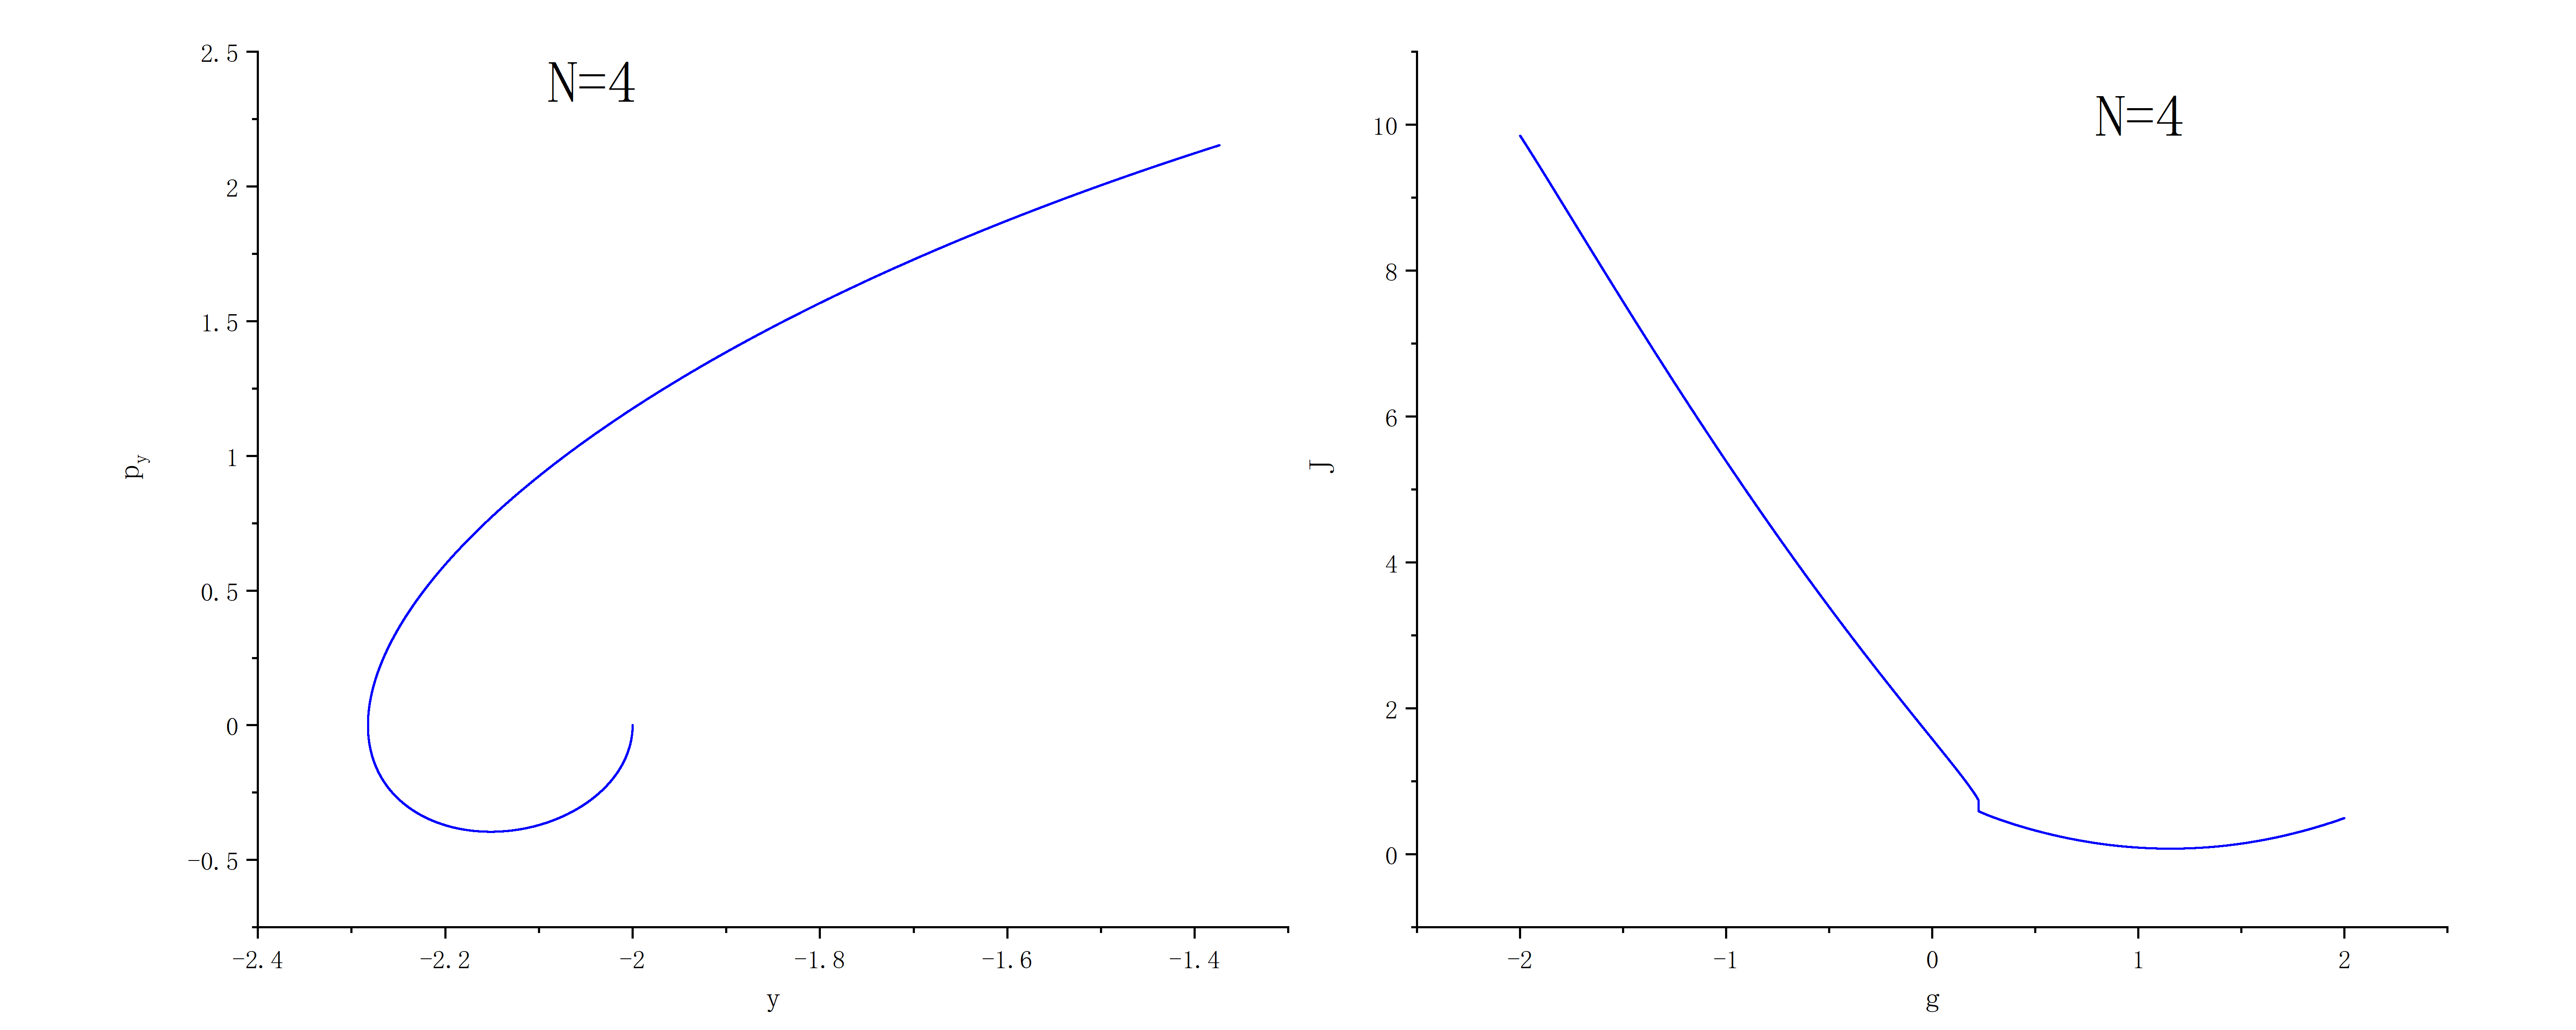
\includegraphics[width=0.9\textwidth]{q3-N=4.jpg}
        \caption{q3-N=4}\label{q3-N=4}
    \end{figure}

    \begin{figure}[H]
        \centering
        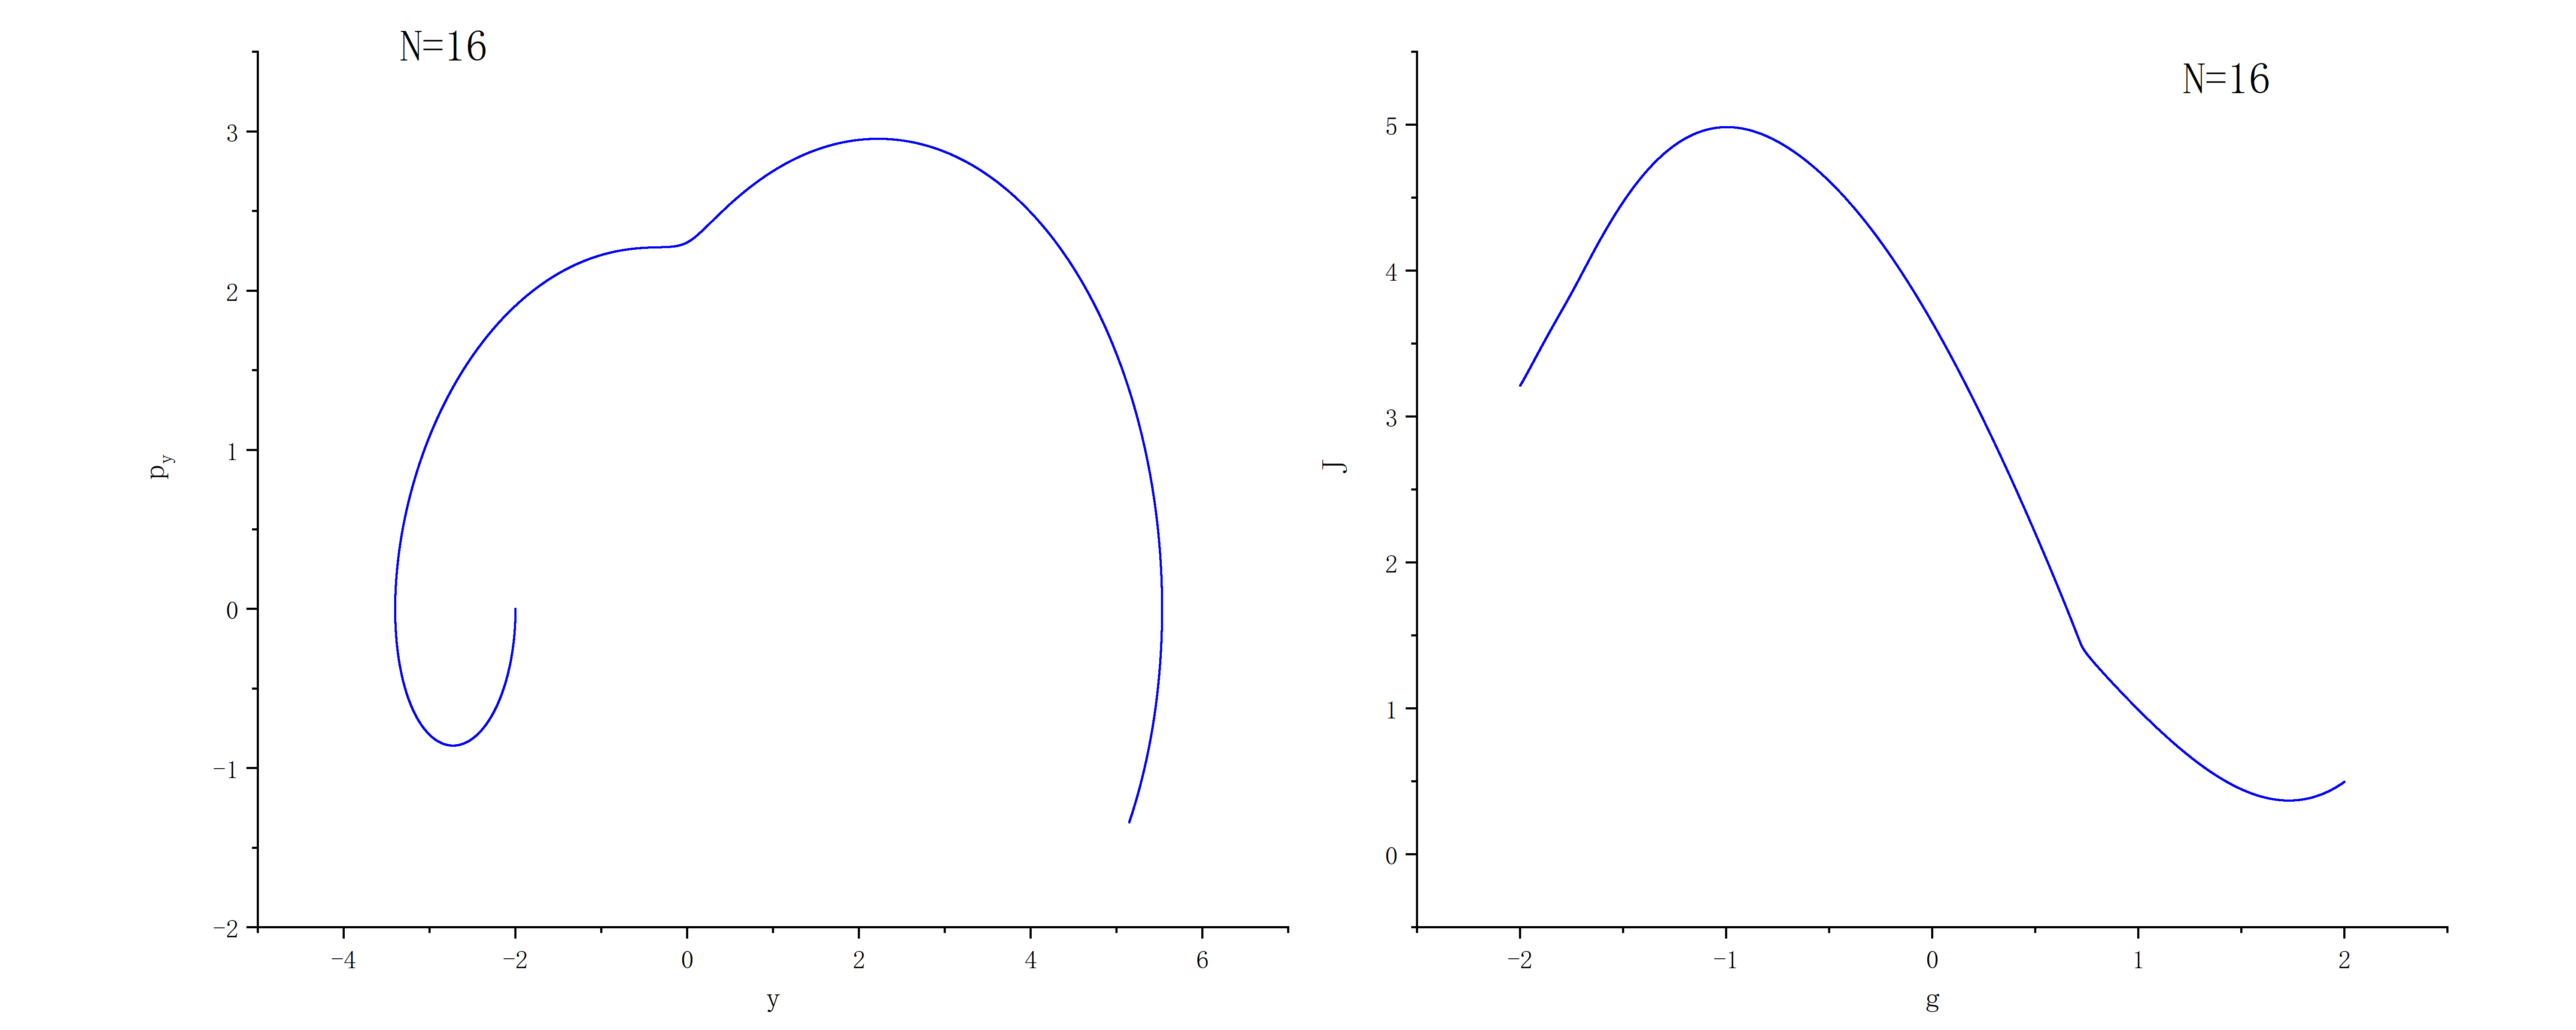
\includegraphics[width=0.9\textwidth]{q3-N=16.jpg}
        \caption{q3-N=16}\label{q3-N=16}
    \end{figure}

    \begin{figure}[H]
        \centering
        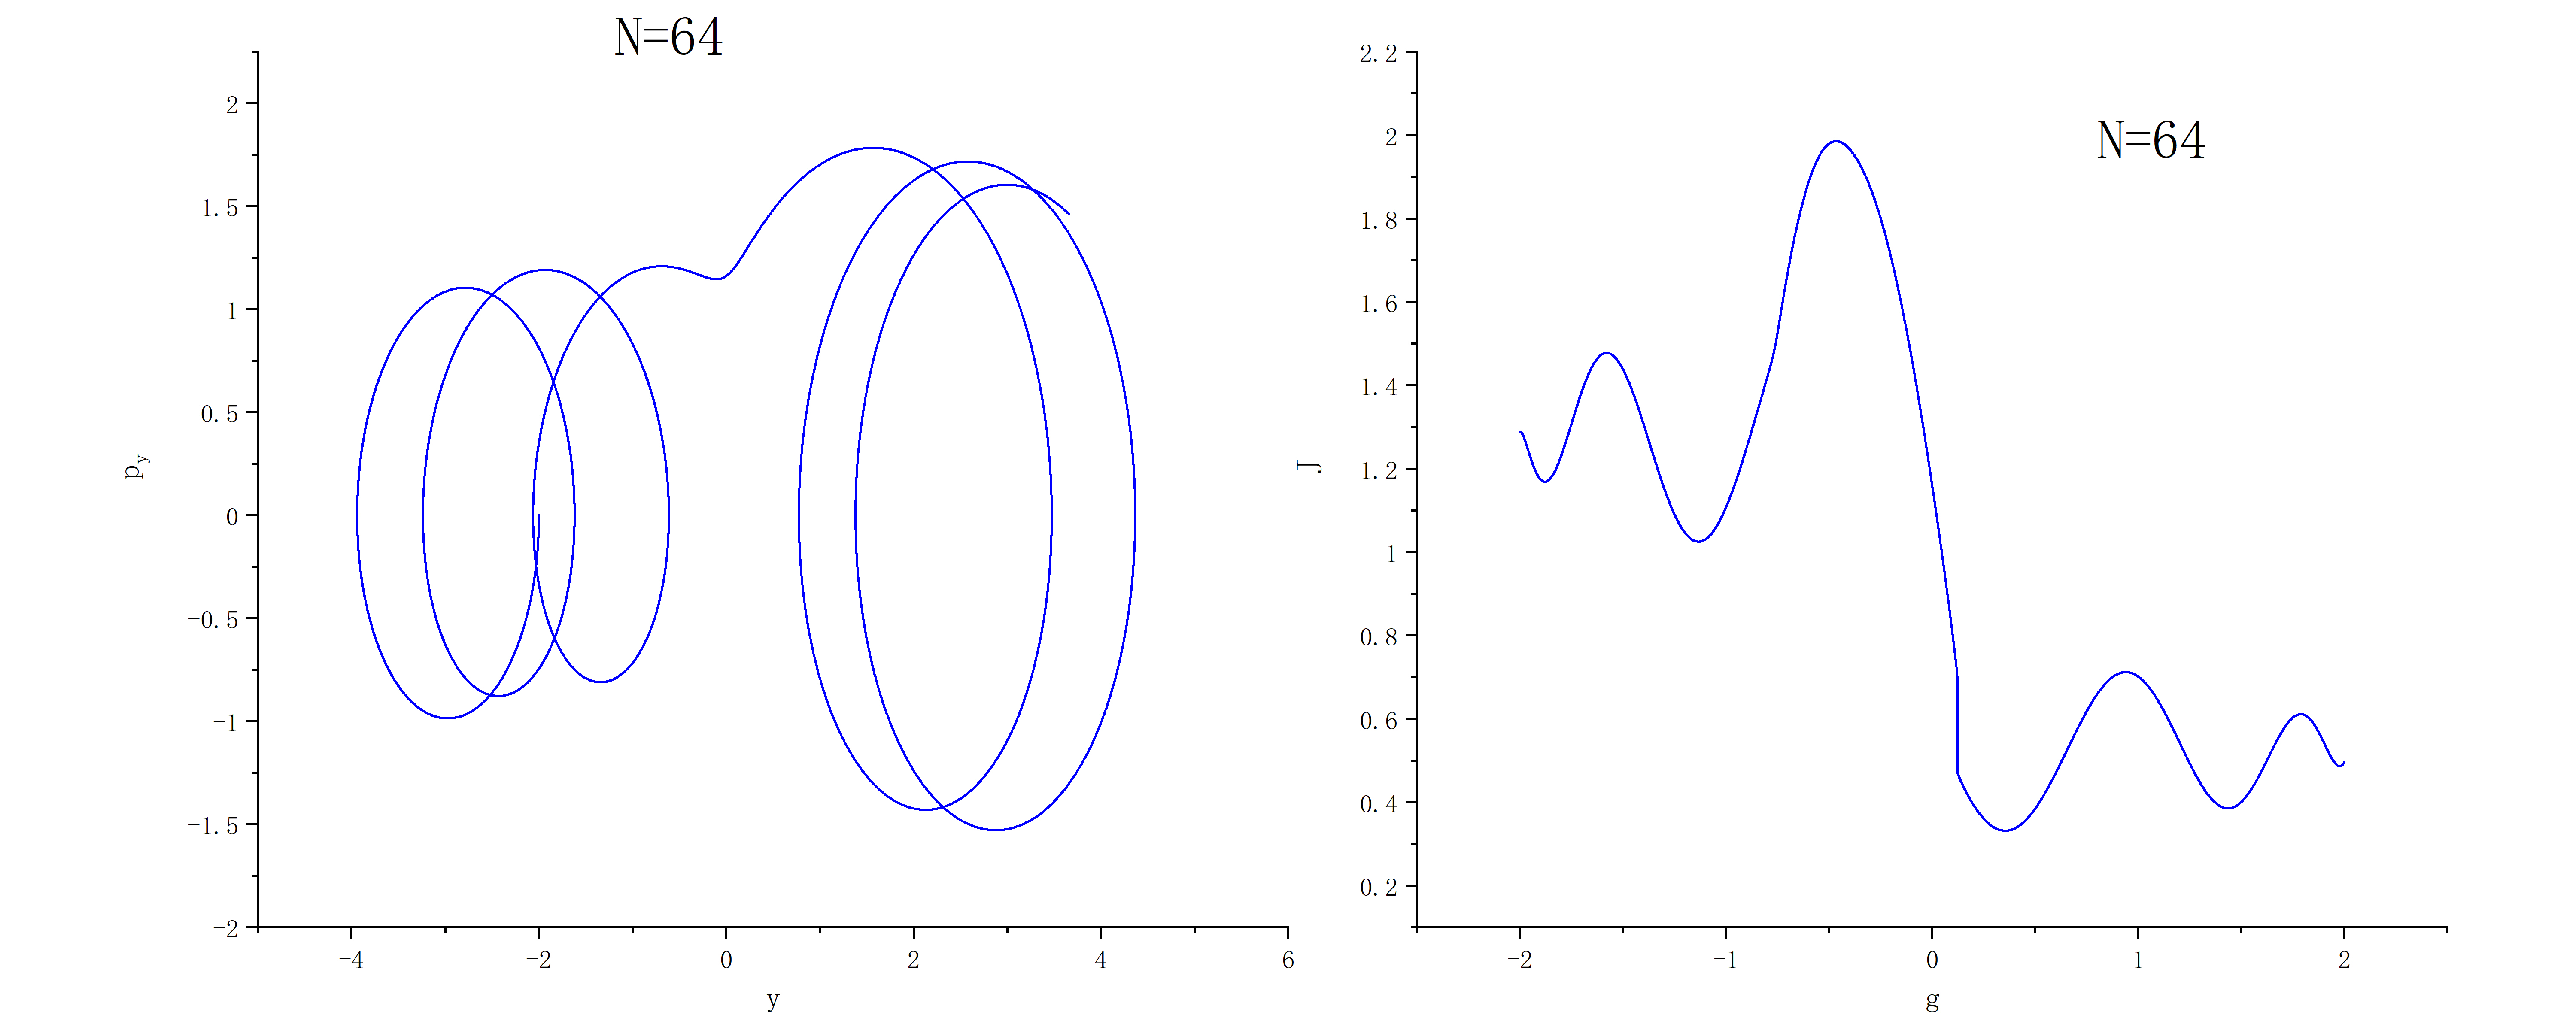
\includegraphics[width=0.9\textwidth]{q3-N=64.jpg}
        \caption{q3-N=64}\label{q3-N=64}
    \end{figure}

    \begin{figure}[H]
        \centering
        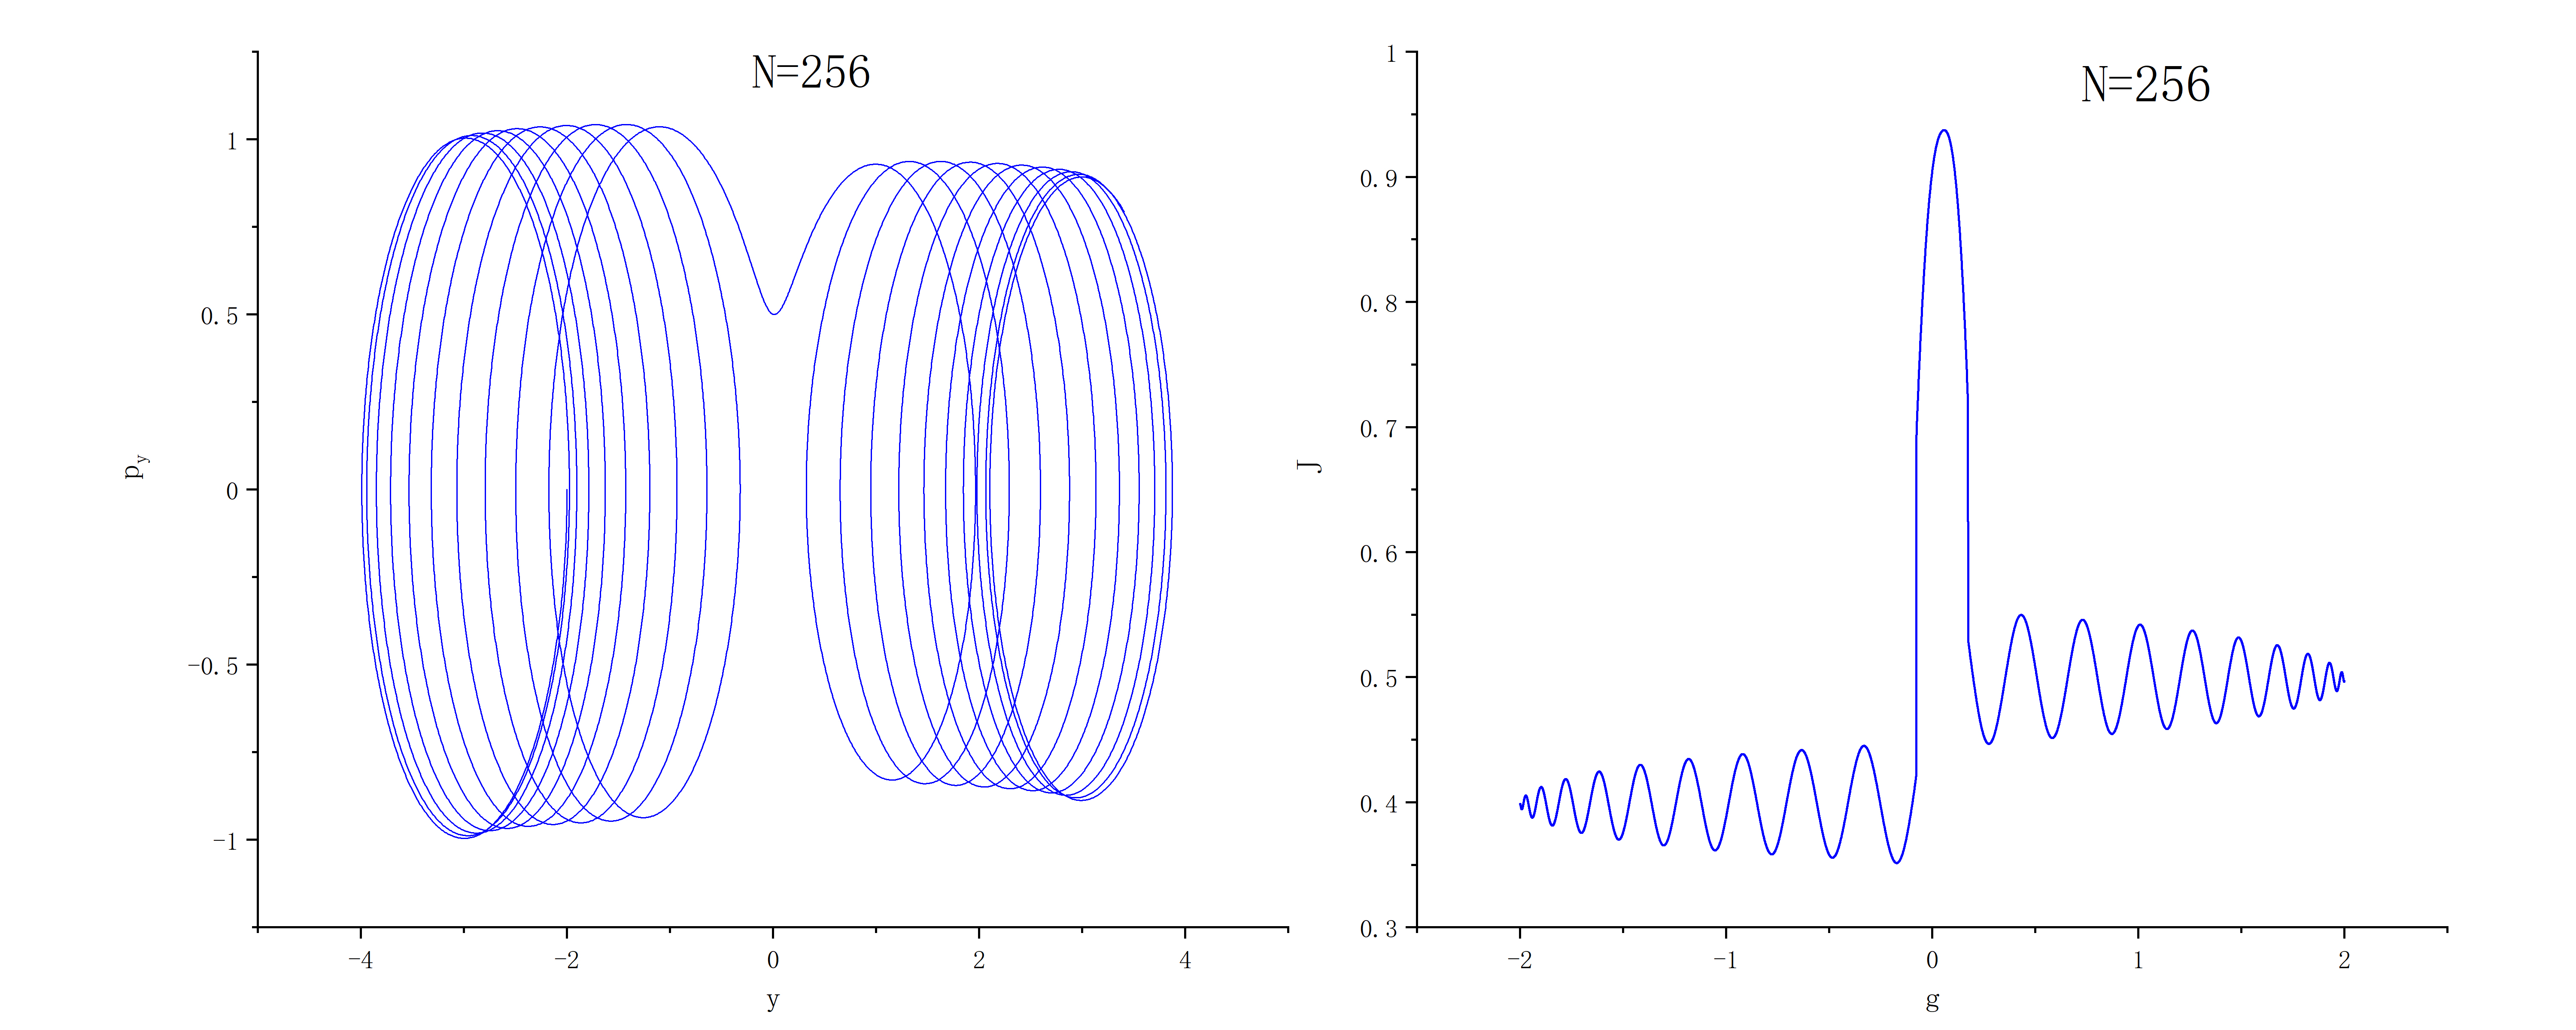
\includegraphics[width=0.9\textwidth]{q3-N=256.jpg}
        \caption{q3-N=256}\label{q3-N=256}
    \end{figure}

    可以看出,当N逐渐变大时(g变化越缓慢),J越趋向于一个不随g变化的常数(可能有阶跃,如图\ref{q3-N=256})。


    \subsection{第4问}

    由于贝瑞相位需要计算$\omega(t)$对t的积分,我们需要先细分t的区间,打出不同t处系统的运动角频率,再用矩形法即可求解。

    本问条件是初始条件:$\wpy_0=0,\wy_0=-2.1$

    缓变参数:$\wg=2\cos(2\pi t/N),\wx=2\sin(2\pi t/N)$

    \subsubsection{计算方法}

    与第2、3问完全相同,应用蛙跳法可以得到体系的相轨。同时得到任意时刻$\wt$冻结x,g时振子的坐标和动量$\wy_0,\wpy_0$,我们将利用它们求解振子振动
    的周期$T(\wt)$,进而通过$\omega(\wt)=\frac{2\pi}{T(\wt)}$得到体系运动角频率。

    求解周期与求解绝热不变量是类似的,相似性可以由表达式看出:

    \begin{align}
        \widetilde{J}&=\frac{1}{2\pi}\oint\wpy d\wy  &  \widetilde{T}=\oint\frac{d\wy}{\wpy}
    \end{align}

    完全类似于绝热不变量的求解,我们先根据初值条件计算总能量H,再解出H和势函数的交点坐标$y_1,y_2$,于是可以计算周期
    \begin{align}
        T=2\int_{y_1}^{y_2}\frac{d\wy}{\wpy}
    \end{align}

    不同的是,在积分上下限上,$\wpy=0$,因此这是一个瑕积分,需要应用切比雪夫积分法。

    根据第2、3问的探索,笔者发现N=256时J就已经近似不随x和g变化了,因此我们在4、5问中都选取N大于等于256。

    我们可以取$t_i=0$数值计算贝瑞相位$\varphi_B$。其中贝瑞相位的第二项可以由矩形法给出,而第一项需要我们知道$p_f,q_f$。

    对N=256的情形,我们已经可以算出

    \begin{align}
        t_i&=0& \wy_i&=-2.1& \wpy_i&=0\\
        t_f&=256& \wy_f&=-2.201021443214239& \wpy_f&=0.414659804187784
    \end{align}

    0时刻g=2,x=0,这时体系平衡位置在-3,说明振子先下落后上升,还差一点点到达一整个周期,这时到达末相位点。

    数值求解这段时间,需要计算一个两端有瑕点的瑕积分,加上一个一侧有瑕点的瑕积分,同样可以利用切比雪夫积分法。

    \subsubsection{结果展示}

    具体代码实现见附录,输出数据见"q4-berry-N=256.txt"

    这是时间t变化一个周期的相图和w-t图

    \begin{figure}[H]
        \centering
        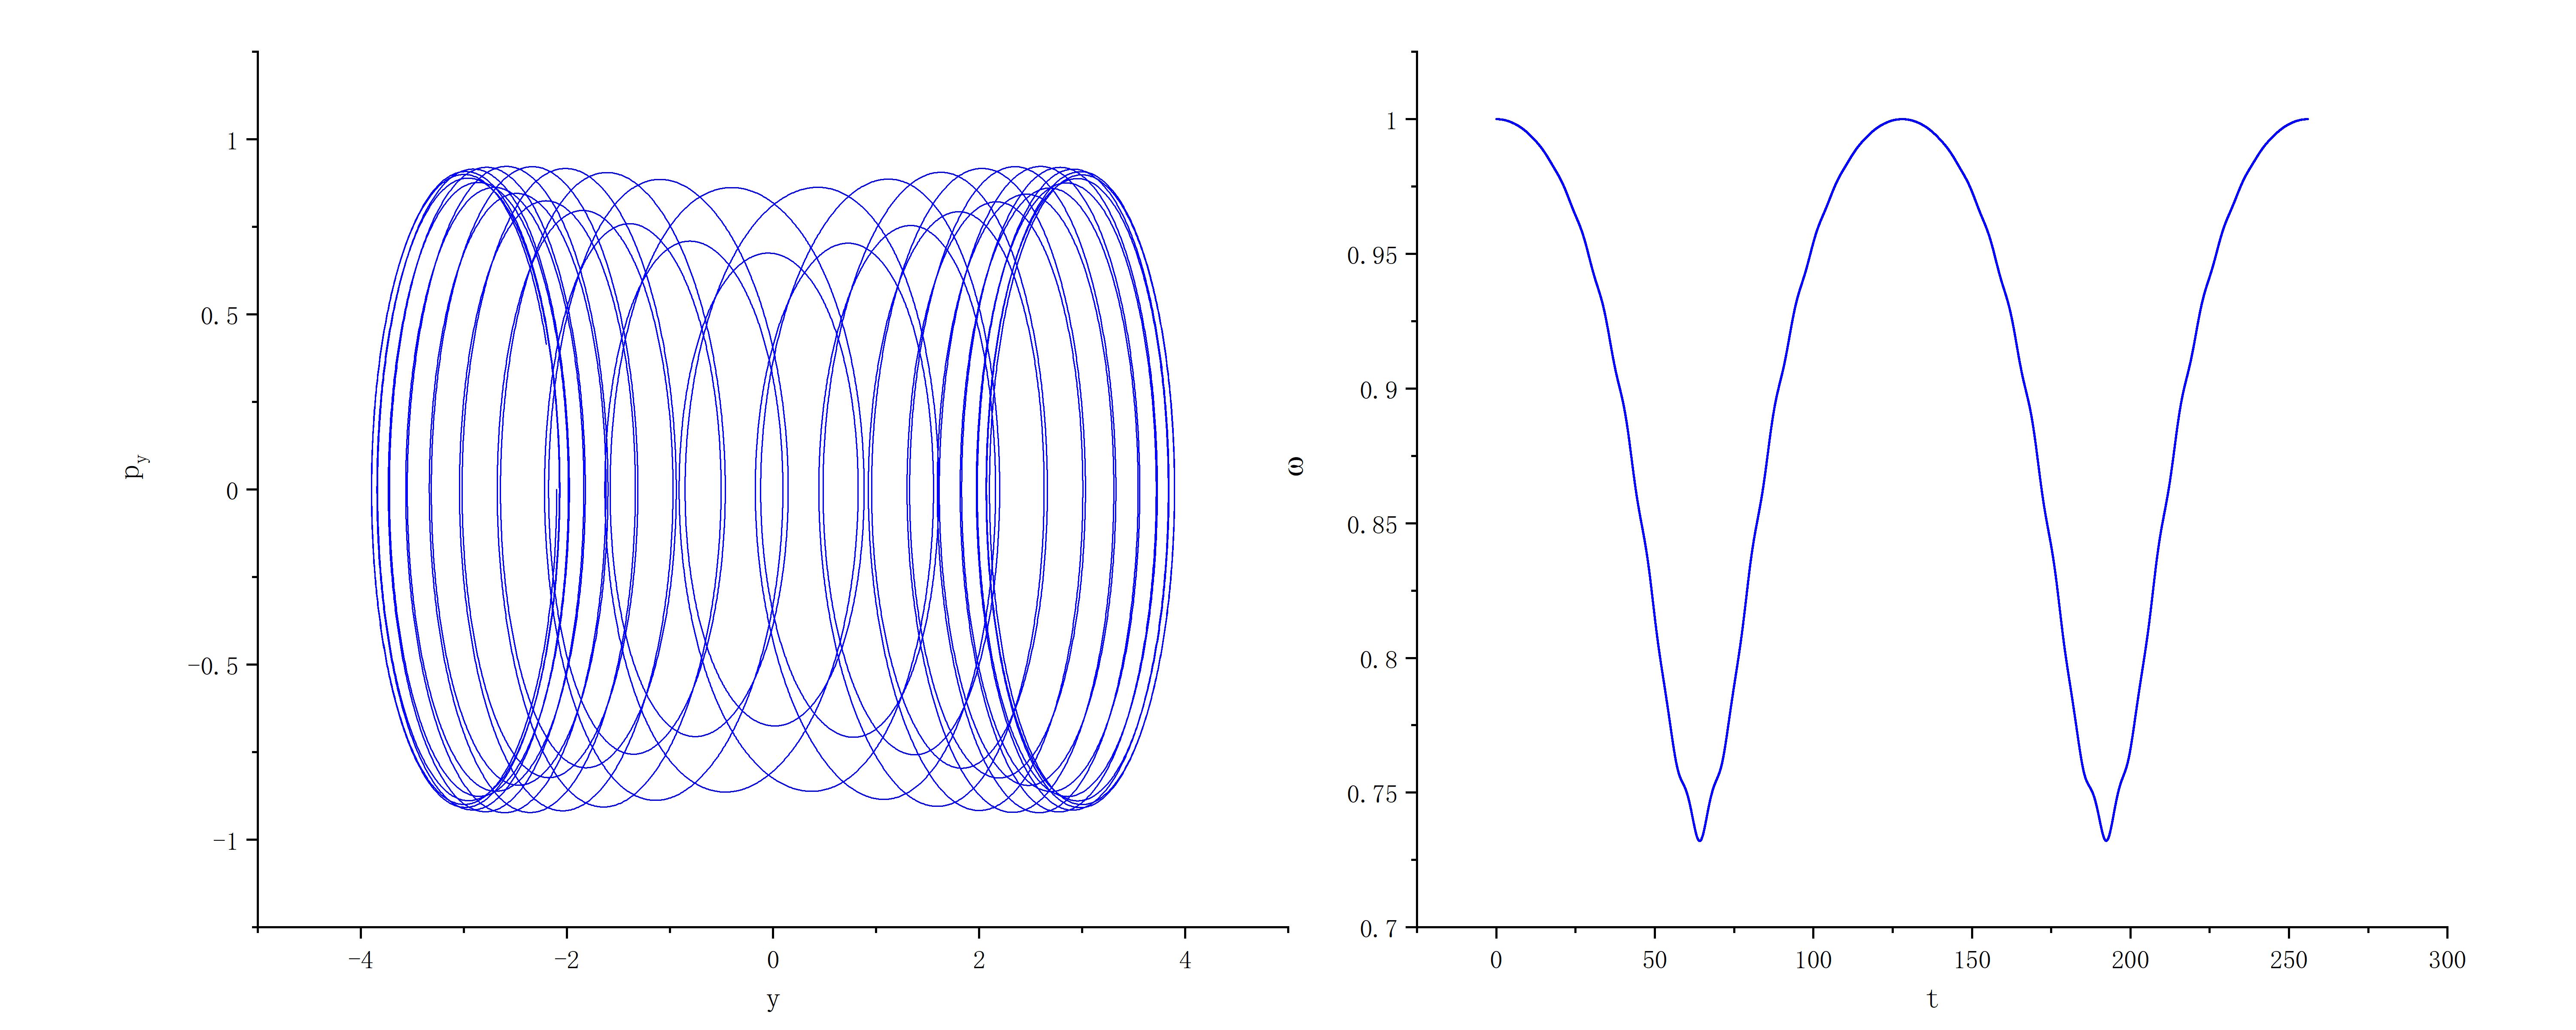
\includegraphics[width=0.9\textwidth]{q4相图及w-t图.jpg}
        \caption{q4相图及w-t图}\label{q4相图及w-t图}
    \end{figure}

    得到
    \begin{align}
        \omega(0)\int_{(p_i,q_i)}^{(p_f,q_f)}dt&\triangleq I_1=5.804463\\
        \int_{t_i}^{t_f}\omega(t)dt&\triangleq I_2=231.974820\\
        \frac{I_1-I_2}{2\pi}&=-35.996\approx-37\\
        \Longrightarrow \phi_B\approx0
    \end{align}

    \subsection{第5问}

    本问条件是初始条件:$\wpy_0=0,\wy_0=0.52$

    缓变参数:$\wg=0.3\cos(2\pi t/N),\wx=0.3\sin(2\pi t/N)$

    本问相较前问的唯一区别在于势函数一直有两个极值,进而在求积分上下限的时候会麻烦一点,方法同第三问的处理。

    我们同样可以取$t_i=0$数值计算贝瑞相位$\varphi_B$。
    类似前问的方法,对N=256的情形,我们已经可以算出

    \begin{align}
        t_i&=0& \wy_i&=0.52 & \wpy_i&=0\\  
        t_f&=256& \wy_f&=0.860848250836850& \wpy_f&=-0.080528416363538
    \end{align}

    0时刻g=0.3,x=0,这时体系平衡位置在+0.7,说明振子由静止先上升后下降,刚刚下降一点,就到达末相位点。

    数值求解这段时间,需要计算一个两端有瑕点的瑕积分,加上一个一侧有瑕点的瑕积分,笔者采用切比雪夫积分法。

    \subsubsection{结果展示}

    具体代码实现见附录,输出数据见"q5-berry-N=256.txt"

    这是时间t变化一个周期的相图和w-t图

    \begin{figure}[H]
        \centering
        \includegraphics[width=0.9\textwidth]{q5相图及w-t图.jpg}
        \caption{q5相图及w-t图}\label{q5相图及w-t图}
    \end{figure}

    得到
    \begin{align}
        \omega(0)\int_{(p_i,q_i)}^{(p_f,q_f)}dt&\triangleq I_1=3.605759 \\
        \int_{t_i}^{t_f}\omega(t)dt&\triangleq I_2=248.651083\\
        \frac{I_1-I_2}{2\pi}&=-39.0002\approx-39\\
        \Longrightarrow \phi_B\approx0
    \end{align}


    \section{附录}
    \subsection{第1问源代码}
    \begin{lstlisting}[language=C]
        #include <stdio.h>
        #include <math.h>
        #define EPS 10e-15
        #define ITV 1e-4
        double x;//参数x从0变到1

        double f(double y){
            double f=pow(y*y+x*x,3)-pow(x,4);
            return f;
        }
        int isInside(double a,double b,double x){//判断x是否在a,b之间
            if((a<x&&x<b)||(b<x&&x<a))return 1;
            else return 0;
        }
        //Dekker method to find root of f(x) in given range [x1,x2]
        double DekkerRoot (double x1,double x2){
            double a=x1,b=x2;
            double temp,m,s,fa,fb;
            if(f(a)*f(b)>0){
                return -404404;
            }
            if(fabs(f(b))>fabs(f(a))){
                temp=a;
                a=b;
                b=temp;
            }
            fa=f(a);
            fb=f(b);

            while(fb!=0&&fabs(a-b)>EPS){
                m=(a+b)/2;
                if(fa!=fb){
                    s=(a*fb-b*fa)/(fb-fa);
                    if(isInside(m,b,s)&&fabs(f(s))<fabs(fb)){
                        if(fb*f(s)<0){
                            a=b;fa=fb;
                            b=s;fb=f(s);
                        }
                        else{
                            b=s;fb=f(s);
                            if(fb*f(m)<0){
                                a=m;fa=f(m);
                            }
                        }
                    }
                    else{
                        pos_1:
                        if(f(m)*fb<0){
                            a=m;
                            fa=f(m);
                        }
                        else{
                            b=m;
                            fb=f(m);
                        }
                    }
                }
                else goto pos_1;

                if(fabs(fb)>fabs(fa)){
                    temp=b;b=a;a=temp;
                    temp=fb;fb=fa;fa=temp;
                }
            }
            return b;
        }

        int main(){
            FILE *fdata=fopen("C://C_files//HW2//plot_x-g_data.txt","w");
            if(fdata==NULL){
                return 0;
            }
            double y,g;
            for ( x = ITV; x < 1; x+=ITV)
            {
                y=DekkerRoot(0,1);//计算切点
                if(y==-404404){
                    fprintf(fdata,"x=%lf, Wrong section!\n",x);
                    continue;
                }
                g=y/(sqrt(x*x+y*y))-y;//将切点回代,得到临界g
                fprintf(fdata,"%lf %.15lf %lf\n",x,y,g);
                printf("%lf\n",x);
            }
            fclose(fdata);
            return 0;
        }
    \end{lstlisting}

    \subsection{第2问源代码}
    为保证迭代精度,笔者手动调节N和dt,对应关系见下表。

    % Table generated by Excel2LaTeX from sheet 'Sheet1'
    \begin{table}[htbp]
        \centering
        \begin{tabular}{|c|c|c|c|c|}\hline
        N     & 4     & 16    & 64    & 256 \\\hline
        dt    &   $1\times10^{-4}$    &    $5\times10^{-4}$   &    $2\times10^{-3}$   & $1\times10^{-2}$ \\\hline
        \text{输出文件}   &    $"q2-1.txt"$   &    $"q2-2.txt"$   &    $"q2-3.txt"$   & $"q2-4.txt"$ \\\hline
        \end{tabular}%
    \end{table}%
  
    \begin{lstlisting}[language=C]
        #include <stdio.h>
        #include <math.h>
        #define EPS_ITG 1e-8//积分特征精度
        #define EPS_ROOT 1e-14//求根特征精度
        #define PI 3.1415926535897932
        double N=4;//v=1/N
        double dt=1e-4;//迭代步长
        double Y_0=0.1;//储存每个时刻的初值位置
        double PY_0=0;//储存每个时刻的初值动量
        double Y_o,Y_n,PY_o,PY_n;//迭代参数
        double xt;//xt=x(t)
        double x(double t);//给定t,返回x值
        double pySquare(double y);//计算给定位置动量的平方
        int isInside(double a,double b,double x);
        double DekkerPySquare(double a, double b);//Dekker算法求pySquare函数零点
        double py(double y);//计算给定位置的动量
        double integrate_phaseSpace(double y1,double y2);//相空间定上下限积分
        double getJ();//计算J

        int main(){
            FILE *fdata=fopen("C://C_files//HW2//q2-1.txt","w");
            if(fdata==NULL){
                return 0;
            }
            Y_n=Y_0;
            PY_n=PY_0+dt/2*(Y_0+dt/4*PY_0)*(-1+1/sqrt(pow(x(1/4*dt),2)
        +pow(Y_0+dt/4*PY_0,2)));
            xt=x(0);
            double J;
            J=getJ();
            fprintf(fdata,"%lf  %lf %lf %lf\n",Y_0,PY_0,x(0),J);
            printf("%lf\n",x(0));//控制台查看运行进度
            double t=dt;
            xt=x(t);
            while(!(xt<0)){//蛙跳法
                Y_o=Y_n;
                PY_o=PY_n;
                Y_n=Y_o+dt*PY_o;
                PY_n=PY_o+dt*Y_n*(-1+1/sqrt(xt*xt+Y_n*Y_n));
                Y_0=Y_n;
                PY_0=(PY_n+PY_o)/2;
                J=getJ();
                fprintf(fdata,"%lf  %lf %lf %lf\n",Y_0,PY_0,xt,J);
                printf("%lf\n",xt);//控制台查看运行进度,无特别含义

                t+=dt;
                xt=x(t);
            }
            fclose(fdata);
            return 0;
        }

        double x(double t){
            if(t<0)return -404404;
            return 2-t/N;
        }

        double pySquare(double y){
            double pySquare=Y_0*Y_0-y*y+2*(sqrt(xt*xt+y*y)
        -sqrt(xt*xt+Y_0*Y_0))+PY_0*PY_0;
            return pySquare;
        }

        int isInside(double a,double b,double x){//判断x是否在a,b之间
            if((a<x&&x<b)||(b<x&&x<a))return 1;
            else return 0;
        }

        double DekkerPySquare(double a, double b){//返回正根,若区间错误返回-1
            double temp,m,s,fa,fb;
            if(pySquare(a)*pySquare(b)>0)return -1;
            if(fabs(pySquare(b))>fabs(pySquare(a))){
                temp=a;
                a=b;
                b=temp;
            }
            fa=pySquare(a);
            fb=pySquare(b);

            while(fabs(fb)>EPS_ROOT&&fabs(a-b)>EPS_ROOT){
                m=(a+b)/2;
                if(fa!=fb){
                    s=(a*fb-b*fa)/(fb-fa);
                    if(isInside(m,b,s)&&fabs(pySquare(s))<fabs(fb)){
                        if(fb*pySquare(s)<0){
                            a=b;fa=fb;
                        }
                        b=s;fb=pySquare(s);
                    }
                    else{
                        pos_1:
                        if(pySquare(m)*fb<0){
                            a=m;
                            fa=pySquare(m);
                        }
                        else{
                            b=m;
                            fb=pySquare(m);
                        }
                    }
                }
                else goto pos_1;

                if(fabs(fb)>fabs(fa)){
                    temp=b;b=a;a=temp;
                    temp=fb;fb=fa;fa=temp;
                }
            }
            return b;
        }
        double py(double y){
            double py_pingfang=pySquare(y);
            double py;
            //由于求积分上下限精度有限,有可能在积分过程中遇到一个y值
            //动量平方是个很小的负数,这时不妨将它抹去,于是有下面置零操作
            if(py_pingfang<0)return 0;
            else{
                py=sqrt(py_pingfang);
                return py;
            }
        }
        double integrate_phaseSpace(double y1,double y2){
            double h=fabs(y2-y1);
            double T=h/2*(py(y1)+py(y2));
            double T0=T-1;
            long long n=2;
            while (fabs(T-T0)>EPS_ITG){//二分法求定积分
                T0=T;
                double S=0;
                double dh=h/n;
                long long i;
                for ( i = 0; 2*i+1 < n ; i++)
                {
                    S+=py(y1+(2*i+1)*dh);
                }
                T=S*dh+0.5*T0;
                n*=2;
            }
            return T;
        }
        double getJ(){
            double y0=fabs(Y_0),py0=fabs(PY_0);
            double yc=DekkerPySquare(y0,2.1);//2.1是估计的上界
            double J;
            if(yc<0)return -404404;
            if(y0*y0+2*(xt-sqrt(xt*xt+y0*y0))+py0*py0>0){
                J=2/PI*(integrate_phaseSpace(0,yc));
            }
            else{
                double ym=DekkerPySquare(0,y0);
                if(ym<0)return -404404;
                J=1/PI*(integrate_phaseSpace(ym,yc));
            }
            return J;
        }


    \end{lstlisting}

    \subsection{第3问源代码}
    为保证迭代精度,笔者手动调节N、dt和MAX,对应关系见下表。

    % Table generated by Excel2LaTeX from sheet 'Sheet1'
    \begin{table}[htbp]
        \centering
        \begin{tabular}{|c|c|c|c|c|}\hline
        N     & 4     & 16    & 64    & 256 \\\hline
        dt    &   $1\times10^{-4}$    &    $5\times10^{-4}$   &    $2\times10^{-3}$   & $1\times10^{-2}$ \\\hline
        MAX   & 8  &  8  &  6  &  4  \\\hline  
        \text{输出文件}   &    $"q3-1.txt"$   &    $"q3-2.txt"$   &    $"q3-3.txt"$   & $"q3-4.txt"$ \\\hline
        \end{tabular}%
    \end{table}%
  
    \begin{lstlisting}[language=C]
        #include <stdio.h>
        #include <math.h>
        #define MAX 8//求根的经验上界
        #define EPS_ITG 1e-8//积分特征精度
        #define EPS_ROOT 1e-14//求根特征精度
        #define PI 3.1415926535897932
        #define X 0.2
        #define Y_THRESHOLD 0.277417932961286//Y临界,与X取值有关
        #define G_THRESHOLD 0.53375//g临界,与X取值有关
        double N=16;
        double dt=5e-4;
        double Y_0=-2;//储存初值条件y0
        double PY_0=0;//储存初值条件py0
        double t;
        double Ymin1,Ymax,Ymin2;//储存三极值时的极值点
        double Ymin;//储存单极值时的极值点
        
        double g(double t){//给定t返回g
            double g=2*cos(2*PI*t/N);
            return g;
        }
        
        double eq1(double y){//求势函数极值点需要使用的方程
            double eq1=y/sqrt(X*X+y*y)-y-g(t);
            return eq1;
        }
        
        double pySquare(double y){//py的平方
            double pySquare=PY_0*PY_0+Y_0*Y_0-y*y+2*(sqrt(X*X+y*y)
        -sqrt(X*X+Y_0*Y_0))+2*(Y_0-y)*g(t);
            return pySquare;
        }
        
        double V(double y){//给定y返回体系势能
            double potential=0.5*pow(sqrt(X*X+y*y)-1,2)+y*g(t);
            return potential;
        }
        int isInside(double a,double b,double x){//判断x是否在a,b之间
            if((a<x&&x<b)||(b<x&&x<a))return 1;
            else return 0;
        }
        
        double DekkerExtreme(double a, double b){//若区间错误返回-404404
            double temp,m,s,fa,fb;
            if(eq1(a)*eq1(b)>0)return -404404;
            if(fabs(eq1(b))>fabs(eq1(a))){
                temp=a;
                a=b;
                b=temp;
            }
            fa=eq1(a);
            fb=eq1(b);
        
            while(fabs(a-b)>EPS_ROOT){
                m=(a+b)/2;
                if(fa!=fb){
                    s=(a*fb-b*fa)/(fb-fa);
                    if(isInside(m,b,s)&&fabs(eq1(s))<fabs(fb)){
                        if(fb*eq1(s)<0){
                            a=b;fa=fb;
                            b=s;fb=eq1(s);
                        }
                        else{
                            b=s;fb=eq1(s);
                            if(fb*eq1(m)<0){
                                a=m;fa=eq1(m);
                            }
                        }
        
                    }
                    else{
                        pos_1:
                        if(eq1(m)*fb<0){
                            a=m;
                            fa=eq1(m);
                        }
                        else{
                            b=m;
                            fb=eq1(m);
                        }
                    }
                }
                else goto pos_1;
        
                if(fabs(fb)>fabs(fa)){
                    temp=b;b=a;a=temp;
                    temp=fb;fb=fa;fa=temp;
                }
            }
            return b;
        }
        
        double DekkerPySquare(double a, double b){//若区间错误返回-404404
            double temp,m,s,fa,fb;
            if(pySquare(a)*pySquare(b)>0)return -404404;
            if(fabs(pySquare(b))>fabs(pySquare(a))){
                temp=a;
                a=b;
                b=temp;
            }
            fa=pySquare(a);
            fb=pySquare(b);
        
            while(fabs(a-b)>EPS_ROOT){
                m=(a+b)/2;
                if(fa!=fb){
                    s=(a*fb-b*fa)/(fb-fa);
                    if(isInside(m,b,s)&&fabs(pySquare(s))<fabs(fb)){
                        if(fb*pySquare(s)<0){
                            a=b;fa=fb;
                            b=s;fb=pySquare(s);
                        }
                        else{
                            b=s;fb=pySquare(s);
                            if(fb*pySquare(m)<0){
                                a=m;fa=pySquare(m);
                            }
                        }
                    }
                    else{
                        pos_1:
                        if(pySquare(m)*fb<0){
                            a=m;
                            fa=pySquare(m);
                        }
                        else{
                            b=m;
                            fb=pySquare(m);
                        }
                    }
                }
                else goto pos_1;
        
                if(fabs(fb)>fabs(fa)){
                    temp=b;b=a;a=temp;
                    temp=fb;fb=fa;fa=temp;
                }
            }
            return b;
        }
        
        double py(double y){
            double py_pingfang=pySquare(y);
            double py;
            if(py_pingfang<0)return 0;
            else{
                py=sqrt(py_pingfang);
                return py;
            }
        }
        double integrate_phaseSpace(double y1,double y2){
            double h=fabs(y2-y1);
            double T=h/2*(py(y1)+py(y2));
            double T0=T-1;
            long long n=2;
            while (fabs(T-T0)>EPS_ITG){
                T0=T;
                double S=0;
                double dh=h/n;
                long long i;
                for ( i = 0; 2*i+1 < n ; i++)
                {
                    S+=py(y1+(2*i+1)*dh);
                }
                T=S*dh+0.5*T0;
                n*=2;
            }
            return T;
        }
        
        double getJ(){
            double H=0.5*PY_0*PY_0+0.5*pow(sqrt(X*X+Y_0*Y_0)-1,2)+Y_0*g(t);
            double gt=g(t);
            double y1,y2;
            double J;
            if(fabs(gt)<0.53375){//势函数双极值
                Ymin1=DekkerExtreme(Y_THRESHOLD,1.6);
                Ymin2=DekkerExtreme(-1.6,-Y_THRESHOLD);
                if(gt>0)Ymax=DekkerExtreme(0,Y_THRESHOLD);
                else Ymax=DekkerExtreme(-Y_THRESHOLD,0);
        
                if(Ymin1<-100||Ymin2<-100||Ymax<-100)return -404404;
        
                if(H>V(Ymax)){
                    y1=DekkerPySquare(-MAX,Ymin2);
                    y2=DekkerPySquare(Ymin1,MAX);
                }
                else{
                    if(Y_0>Ymax){
                        y1=DekkerPySquare(Ymax,Ymin1);
                        y2=DekkerPySquare(Ymin1,MAX);
                    }
                    else{
                        y1=DekkerPySquare(-MAX,Ymin2);
                        y2=DekkerPySquare(Ymin2,Ymax);
                    }
                }
            }
            else{//势函数单极值
                if(gt>0){
                    Ymin=DekkerExtreme(-3,0);
                }
                else Ymin=DekkerExtreme(0,3);
        
                if(Ymin<-100)return -404404;
                
                if(H>V(Ymin)){
                    y1=DekkerPySquare(-MAX,Ymin);
                    y2=DekkerPySquare(Ymin,MAX);
                }
                else return 0;
            }
            if(y1<-100||y2<-100)return -404404;
        
            J=1/PI*integrate_phaseSpace(y1,y2);
        
            return J;
        }
        int main(){
            FILE *fdata=fopen("C://C_files//HW2//q3-2.txt","w");
            if(fdata==NULL){
                return 0;
            }
            double y_o,y_n,py_o,py_n;
            y_n=Y_0;
            py_n=PY_0+dt/2*((Y_0+dt/4*PY_0)*
        (-1+1/sqrt(X*X+pow(Y_0+dt/4*PY_0,2)))-g(dt/4));
            t=0;
            double J;
            J=getJ();
            fprintf(fdata,"%.15lf  %.15lf %lf %lf\n",Y_0,PY_0,g(t),J);
            printf("%lf\n",g(t));//控制台输出一个g值,方便查看进度
            
            
            for(t=dt;t<=N/2;t+=dt){//蛙跳法
                y_o=y_n;
                py_o=py_n;
                y_n=y_o+dt*py_o;
                py_n=py_o+dt*(y_n*(-1+1/sqrt(X*X+y_n*y_n))-g(t));
                Y_0=y_n;
                PY_0=(py_n+py_o)/2;
                J=getJ();
                fprintf(fdata,"%.15lf  %.15lf %lf %lf\n",Y_0,PY_0,g(t),J);
                printf("%lf\n",g(t));//控制台输出一个g值,方便查看进度
            }
            fclose(fdata);
            return 0;
        }

    \end{lstlisting}

    \subsection{第4问源代码}
  
    \begin{lstlisting}[language=C]
        //本程序输出第五问条件下相轨数据点、w(t)数据点,
        //和t=0贝瑞相位计算值
        #include <stdio.h>
        #include <math.h>
        #include <limits.h>
        #define EPS_ITG 1e-8
        #define EPS_ROOT 1e-15
        #define PI 3.1415926535897932

        double N=256;
        double dt=1e-2;
        double Y_0=-2.1;
        double PY_0=0;
        double t,xt,gt;
        double Ymin;

        double g(double t){
            double g=2*cos(2*PI*t/N);
            return g;
        }

        double x(double t){
            double x=2*sin(2*PI*t/N);
            return x;
        }

        double eq1(double y){
            double eq1=y/sqrt(xt*xt+y*y)-y-gt;
            return eq1;
        }

        double pySquare(double y){
            double pySquare=PY_0*PY_0+Y_0*Y_0-y*y+2*(sqrt(xt*xt+y*y)
        -sqrt(xt*xt+Y_0*Y_0))+2*(Y_0-y)*gt;
            return pySquare;
        }

        double V(double y){//给定y返回体系势能
            double potential=0.5*pow(sqrt(xt*xt+y*y)-1,2)+y*gt;
            return potential;
        }

        int isInside(double a,double b,double x){//判断x是否在a,b之间
            if((a<x&&x<b)||(b<x&&x<a))return 1;
            else return 0;
        }

        double DekkerRoot(double a, double b,double(*f)(double y)){
            //若区间错误返回-404404
            double temp,m,s,fa,fb;
            if((*f)(a)*(*f)(b)>0)return -404404;
            if(fabs((*f)(b))>fabs((*f)(a))){
                temp=a;
                a=b;
                b=temp;
            }
            fa=(*f)(a);
            fb=(*f)(b);

            while(fb!=0&&fabs(a-b)>EPS_ROOT){
                m=(a+b)/2;
                if(fa!=fb){
                    s=(a*fb-b*fa)/(fb-fa);
                    if(isInside(m,b,s)&&fabs((*f)(s))<fabs(fb)){
                        if(fb*(*f)(s)<0){
                            a=b;fa=fb;
                            b=s;fb=(*f)(s);
                        }
                        else{
                            b=s;fb=(*f)(s);
                            if(fb*(*f)(m)<0){
                                a=m;fa=(*f)(m);
                            }
                        }
                    }
                    else{
                        pos_1:
                        if((*f)(m)*fb<0){
                            a=m;
                            fa=(*f)(m);
                        }
                        else{
                            b=m;
                            fb=(*f)(m);
                        }
                    }
                }
                else goto pos_1;

                if(fabs(fb)>fabs(fa)){
                    temp=b;b=a;a=temp;
                    temp=fb;fb=fa;fa=temp;
                }
            }
            //由于积周期的时候不可以出现分母为0的情况,即不允许py()函数置零
            //需要这里必须解出正根,因此这里对Dekker算法做了小变动
            //这里将输出方程值为正数的近似根,根据判断条件,与Dekker算法给出的
            //近似根不会差出EPS_ROOT以上,依然能够保证精度
            if(fb>=0)return b;
            else return a;
            
        }

        double py(double y){
            double py_pingfang=pySquare(y);
            double py;
            if(py_pingfang<0)return 0;
            else{
                py=sqrt(py_pingfang);
                return py;
            }
        }

        double integratePeriod(double y1,double y2){//两端瑕点的瑕积分
            double T=0,T0=-1;
            double yi;
            int n,i;
            for ( n = 1; fabs(T-T0)>EPS_ITG; n++)
            {
                double S=0;
                for ( i = 0; i < n; i++)
                {
                    yi=(y1+y2)/2+(y2-y1)/2*cos((2*i+1)*PI/(2*n));
                    S+=sqrt((y2-yi)*(yi-y1))/py(yi);
                }
                T0=T;
                T=S*PI/n;
            }
            return T;
        }
        //左端点瑕点的瑕积分
        double integratePeriod_left_infty(double y1,double y2,double y){
            double T=0,T0=-1;
            double yi;
            if(!isInside(y1,y2,y))return -404404;
            double y_sum=(y1+y2)/2,y_minus=(y2-y1)/2;
            double h=acos((y_sum-y)/y_minus);
            int n,i;
            for ( n = 1; fabs(T-T0)>EPS_ITG; n++)
            {
                double S=0;
                for ( i = 0; i < n; i++)
                {
                    yi=(y1+y2)/2+(y2-y1)/2*cos((2*i+1)*h/(2*n));
                    S+=sqrt((y2-yi)*(yi-y1))/py(yi);
                }
                T0=T;
                T=S*h/n;
            }
            return T;
        }

        double getW(void){
            double H=0.5*PY_0*PY_0+0.5*pow(sqrt(xt*xt+Y_0*Y_0)-1,2)+gt*Y_0;
            Ymin=DekkerRoot(-3,3,eq1);
            if(Ymin<-100)return -404404;
            if(H<V(Ymin))return -404;

            double y1,y2;//相空间积分上下限
            y1=DekkerRoot(-8,Ymin,pySquare);
            y2=DekkerRoot(Ymin,8,pySquare);
            printf("%.15lf %.15lf\n",pySquare(y1),pySquare(y2));
            double T;//周期
            T=2*integratePeriod(y1,y2);
            if(T==0)return INT_MAX;
            double w=2*PI/T;
            return w;
        }

        int main(){
            FILE *fdata=fopen("C://C_files//HW2//q4-berry-N=2048.txt","w");
            if(fdata==NULL){
                return 0;
            }
            double y_o,y_n,py_o,py_n;
            double I1,I2=0;
            double wi,yi,pyi,yf,pyf;
            yi=Y_0;pyi=PY_0;
            double w;
            y_n=Y_0;
            py_n=PY_0+dt/2*((Y_0+dt/4*PY_0)*(-1+1/sqrt(x(dt/4)*x(dt/4)
        +pow(Y_0+dt/4*PY_0,2)))-g(dt/4));
            t=0;xt=x(t);gt=g(t);
            w=getW();
            wi=w;
            fprintf(fdata,"%.15lf  %.15lf %lf %lf\n",Y_0,PY_0,t,w);
            
            
            for(t=dt;t<N;t+=dt){//蛙跳法求相图及w(t)
                xt=x(t);
                gt=g(t);
                y_o=y_n;
                py_o=py_n;
                y_n=y_o+dt*py_o;
                py_n=py_o+dt*(y_n*(-1+1/sqrt(xt*xt+y_n*y_n))-gt);
                Y_0=y_n;
                PY_0=(py_n+py_o)/2;
                w=getW();
                I2+=w*dt;
                fprintf(fdata,"%.15lf  %.15lf %lf %lf\n",Y_0,PY_0,t,w);
            }
            yf=Y_0;pyf=PY_0;
            
            //数值计算贝瑞相位
            t=0;xt=x(t);gt=g(t);
            double H=0.5*pyi*pyi+0.5*pow(sqrt(xt*xt+yi*yi)-1,2)+gt*yi;
            Ymin=DekkerRoot(-3,3,eq1);
            if(Ymin<-100)fprintf(fdata,"wrong section\n");
            if(H<V(Ymin))fprintf(fdata,"invalid energy\n");

            double y1,y2;//相空间积分上下限
            y1=DekkerRoot(-8,Ymin,pySquare);
            y2=DekkerRoot(Ymin,8,pySquare);

            I1=wi*(integratePeriod(y1,y2)+integratePeriod_left_infty(y1,y2,yf));

            fprintf(fdata,"%lf %lf %lf\n",I1,I2,(I1-I2)
        -round((I1-I2)/(2*PI))*2*PI);

            fclose(fdata);
            return 0;
        }

    \end{lstlisting}

    \subsection{第3问源代码}
    
    \begin{lstlisting}[language=C]
        //本程序输出第五问条件下相轨数据点、w(t)数据点,
        //和t=0贝瑞相位计算值
        #include <stdio.h>
        #include <math.h>
        #include <limits.h>
        #define MAX 8
        #define EPS_ITG 1e-8
        #define EPS_ROOT 1e-15
        #define PI 3.1415926535897932

        double N=256;
        double dt=1e-2;
        double Y_0=0.52;
        double PY_0=0;
        double t,xt,gt;
        double Ymin1,Ymin2,Ymax;
        double Y_threshold;

        double g(double t){
            double g=0.3*cos(2*PI*t/N);
            return g;
        }

        double x(double t){
            double x=0.3*sin(2*PI*t/N);
            return x;
        }

        double f(double y){
            double f=pow(y*y+xt*xt,3)-pow(xt,4);
            return f;
        }

        double eq1(double y){
            double eq1=y/sqrt(xt*xt+y*y)-y-gt;
            return eq1;
        }

        double pySquare(double y){
            double pySquare=PY_0*PY_0+Y_0*Y_0-y*y+2*(sqrt(xt*xt+y*y)
        -sqrt(xt*xt+Y_0*Y_0))+2*(Y_0-y)*gt;
            return pySquare;
        }

        double V(double y){//给定y返回体系势能
            double potential=0.5*pow(sqrt(xt*xt+y*y)-1,2)+y*gt;
            return potential;
        }

        int isInside(double a,double b,double x){//判断x是否在a,b之间
            if((a<x&&x<b)||(b<x&&x<a))return 1;
            else return 0;
        }

        double DekkerRoot(double a, double b,double(*f)(double y)){
            //若区间错误返回-404404
            double temp,m,s,fa,fb;
            if((*f)(a)*(*f)(b)>0)return -404404;
            if(fabs((*f)(b))>fabs((*f)(a))){
                temp=a;
                a=b;
                b=temp;
            }
            fa=(*f)(a);
            fb=(*f)(b);

            while(fb!=0&&fabs(a-b)>EPS_ROOT){
                m=(a+b)/2;
                if(fa!=fb){
                    s=(a*fb-b*fa)/(fb-fa);
                    if(isInside(m,b,s)&&fabs((*f)(s))<fabs(fb)){
                        if(fb*(*f)(s)<0){
                            a=b;fa=fb;
                            b=s;fb=(*f)(s);
                        }
                        else{
                            b=s;fb=(*f)(s);
                            if(fb*(*f)(m)<0){
                                a=m;fa=(*f)(m);
                            }
                        }
                    }
                    else{
                        pos_1:
                        if((*f)(m)*fb<0){
                            a=m;
                            fa=(*f)(m);
                        }
                        else{
                            b=m;
                            fb=(*f)(m);
                        }
                    }
                }
                else goto pos_1;

                if(fabs(fb)>fabs(fa)){
                    temp=b;b=a;a=temp;
                    temp=fb;fb=fa;fa=temp;
                }
            }
            if(fb>=0)return b;
            else return a;
            
        }

        double py(double y){
            double py_pingfang=pySquare(y);
            double py;
            if(py_pingfang<0)return 0;
            else{
                py=sqrt(py_pingfang);
                return py;
            }
        }

        double integratePeriod(double y1,double y2){
            double T=0,T0=-1;
            double yi;
            int n,i;
            for ( n = 1; fabs(T-T0)>EPS_ITG; n++)
            {
                double S=0;
                for ( i = 0; i < n; i++)
                {
                    yi=(y1+y2)/2+(y2-y1)/2*cos((2*i+1)*PI/(2*n));
                    S+=sqrt((y2-yi)*(yi-y1))/py(yi);
                }
                T0=T;
                T=S*PI/n;
            }
            return T;
        }
        //右端点瑕点的瑕积分
        double integratePeriod_right_infty(double y1,double y2,double y){
            double T=0,T0=-1;
            double yi;
            if(!isInside(y1,y2,y))return -404404;
            double y_sum=(y1+y2)/2,y_minus=(y2-y1)/2;
            double h=acos((y-y_sum)/y_minus);
            int n,i;
            for ( n = 1; fabs(T-T0)>EPS_ITG; n++)
            {
                double S=0;
                for ( i = 0; i < n; i++)
                {
                    yi=(y1+y2)/2+(y2-y1)/2*cos((2*i+1)*h/(2*n));
                    S+=sqrt((y2-yi)*(yi-y1))/py(yi);
                }
                T0=T;
                T=S*h/n;
            }
            return T;
        }

        double getW(void){
            double H=0.5*PY_0*PY_0+0.5*pow(sqrt(xt*xt+Y_0*Y_0)-1,2)+gt*Y_0;
            
            if(xt==0){
                Ymax=0;
                Ymin1=DekkerRoot(0,3,eq1);
                Ymin2=DekkerRoot(-3,0,eq1);
            }
            else{
                Y_threshold=DekkerRoot(0,2,f);
                Ymin1=DekkerRoot(Y_threshold,3,eq1);
                Ymin2=DekkerRoot(-3,-Y_threshold,eq1);
                if(gt>0)Ymax=DekkerRoot(0,Y_threshold,eq1);
                else Ymax=DekkerRoot(-Y_threshold,0,eq1);
            }
            if(Ymin1<-100||Ymin2<-100||Ymax<-100||Y_threshold<-100)
            return -404404;
            
            double y1,y2;//相空间积分上下限
            if(H>V(Ymax)){
                    y1=DekkerRoot(-MAX,Ymin2,pySquare);
                    y2=DekkerRoot(Ymin1,MAX,pySquare);
                }
            else{
                if(Y_0>Ymax){
                    y1=DekkerRoot(Ymax,Ymin1,pySquare);
                    y2=DekkerRoot(Ymin1,MAX,pySquare);
                }
                else{
                    y1=DekkerRoot(-MAX,Ymin2,pySquare);
                    y2=DekkerRoot(Ymin2,Ymax,pySquare);
                }
            }

            printf("%.15lf %.15lf\n",pySquare(y1),pySquare(y2));
            double T;//周期
            T=2*integratePeriod(y1,y2);
            if(T==0)return INT_MAX;
            double w=2*PI/T;
            return w;
        }

        int main(){
            FILE *fdata=fopen("C://C_files//HW2//q5-berry-N=256.txt","w");
            if(fdata==NULL){
                return 0;
            }
            double y_o,y_n,py_o,py_n;
            double I1,I2=0;
            double wi,yi,pyi,yf,pyf;
            yi=Y_0;pyi=PY_0;
            double w;
            y_n=Y_0;
            py_n=PY_0+dt/2*((Y_0+dt/4*PY_0)*(-1+1/sqrt(x(dt/4)*x(dt/4)
        +pow(Y_0+dt/4*PY_0,2)))-g(dt/4));
            t=0;xt=x(t);gt=g(t);
            w=getW();
            wi=w;
            fprintf(fdata,"%.15lf  %.15lf %lf %lf\n",Y_0,PY_0,t,w);
            
            
            for(t=dt;t<N;t+=dt){//蛙跳法
                xt=x(t);
                gt=g(t);
                y_o=y_n;
                py_o=py_n;
                y_n=y_o+dt*py_o;
                py_n=py_o+dt*(y_n*(-1+1/sqrt(xt*xt+y_n*y_n))-gt);
                Y_0=y_n;
                PY_0=(py_n+py_o)/2;
                w=getW();
                I2+=w*dt;
                fprintf(fdata,"%.15lf  %.15lf %lf %lf\n",Y_0,PY_0,t,w);
            }
            yf=Y_0;pyf=PY_0;
            
            yf=Y_0;pyf=PY_0;
            
            t=0;xt=x(t);gt=g(t);
            double H=0.5*pyi*pyi+0.5*pow(sqrt(xt*xt+yi*yi)-1,2)+gt*yi;

            if(xt==0){
                Ymax=0;
                Ymin1=DekkerRoot(0,3,eq1);
                Ymin2=DekkerRoot(-3,0,eq1);
            }
            else{
                Y_threshold=DekkerRoot(0,2,f);
                Ymin1=DekkerRoot(Y_threshold,3,eq1);
                Ymin2=DekkerRoot(-3,-Y_threshold,eq1);
                if(gt>0)Ymax=DekkerRoot(0,Y_threshold,eq1);
                else Ymax=DekkerRoot(-Y_threshold,0,eq1);
            }
            if(Ymin1<-100||Ymin2<-100||Ymax<-100||Y_threshold<-100)
            return -404404;
            
            double y1,y2;//相空间积分上下限
            if(H>V(Ymax)){
                    y1=DekkerRoot(-MAX,Ymin2,pySquare);
                    y2=DekkerRoot(Ymin1,MAX,pySquare);
                }
            else{
                if(Y_0>Ymax){
                    y1=DekkerRoot(Ymax,Ymin1,pySquare);
                    y2=DekkerRoot(Ymin1,MAX,pySquare);
                }
                else{
                    y1=DekkerRoot(-MAX,Ymin2,pySquare);
                    y2=DekkerRoot(Ymin2,Ymax,pySquare);
                }
            }

            I1=wi*(integratePeriod(y1,y2)
        +integratePeriod_right_infty(y1,y2,yf));
            fprintf(fdata,"%lf %lf %lf\n",I1,I2,
        (I1-I2)-round((I1-I2)/(2*PI))*2*PI);

            fclose(fdata);
            return 0;
        }

    \end{lstlisting}

\end{document}